% Options for packages loaded elsewhere
% Options for packages loaded elsewhere
\PassOptionsToPackage{unicode}{hyperref}
\PassOptionsToPackage{hyphens}{url}
\PassOptionsToPackage{dvipsnames,svgnames,x11names}{xcolor}
%
\documentclass[
  a4paper,
]{scrreprt}
\usepackage{xcolor}
\usepackage[top=2.5cm, bottom=2.5cm, left=3cm, right=3cm]{geometry}
\usepackage{amsmath,amssymb}
\setcounter{secnumdepth}{5}
\usepackage{iftex}
\ifPDFTeX
  \usepackage[T1]{fontenc}
  \usepackage[utf8]{inputenc}
  \usepackage{textcomp} % provide euro and other symbols
\else % if luatex or xetex
  \usepackage{unicode-math} % this also loads fontspec
  \defaultfontfeatures{Scale=MatchLowercase}
  \defaultfontfeatures[\rmfamily]{Ligatures=TeX,Scale=1}
\fi
\usepackage{lmodern}
\ifPDFTeX\else
  % xetex/luatex font selection
\fi
% Use upquote if available, for straight quotes in verbatim environments
\IfFileExists{upquote.sty}{\usepackage{upquote}}{}
\IfFileExists{microtype.sty}{% use microtype if available
  \usepackage[]{microtype}
  \UseMicrotypeSet[protrusion]{basicmath} % disable protrusion for tt fonts
}{}
\makeatletter
\@ifundefined{KOMAClassName}{% if non-KOMA class
  \IfFileExists{parskip.sty}{%
    \usepackage{parskip}
  }{% else
    \setlength{\parindent}{0pt}
    \setlength{\parskip}{6pt plus 2pt minus 1pt}}
}{% if KOMA class
  \KOMAoptions{parskip=half}}
\makeatother
% Make \paragraph and \subparagraph free-standing
\makeatletter
\ifx\paragraph\undefined\else
  \let\oldparagraph\paragraph
  \renewcommand{\paragraph}{
    \@ifstar
      \xxxParagraphStar
      \xxxParagraphNoStar
  }
  \newcommand{\xxxParagraphStar}[1]{\oldparagraph*{#1}\mbox{}}
  \newcommand{\xxxParagraphNoStar}[1]{\oldparagraph{#1}\mbox{}}
\fi
\ifx\subparagraph\undefined\else
  \let\oldsubparagraph\subparagraph
  \renewcommand{\subparagraph}{
    \@ifstar
      \xxxSubParagraphStar
      \xxxSubParagraphNoStar
  }
  \newcommand{\xxxSubParagraphStar}[1]{\oldsubparagraph*{#1}\mbox{}}
  \newcommand{\xxxSubParagraphNoStar}[1]{\oldsubparagraph{#1}\mbox{}}
\fi
\makeatother


\usepackage{longtable,booktabs,array}
\usepackage{calc} % for calculating minipage widths
% Correct order of tables after \paragraph or \subparagraph
\usepackage{etoolbox}
\makeatletter
\patchcmd\longtable{\par}{\if@noskipsec\mbox{}\fi\par}{}{}
\makeatother
% Allow footnotes in longtable head/foot
\IfFileExists{footnotehyper.sty}{\usepackage{footnotehyper}}{\usepackage{footnote}}
\makesavenoteenv{longtable}
\usepackage{graphicx}
\makeatletter
\newsavebox\pandoc@box
\newcommand*\pandocbounded[1]{% scales image to fit in text height/width
  \sbox\pandoc@box{#1}%
  \Gscale@div\@tempa{\textheight}{\dimexpr\ht\pandoc@box+\dp\pandoc@box\relax}%
  \Gscale@div\@tempb{\linewidth}{\wd\pandoc@box}%
  \ifdim\@tempb\p@<\@tempa\p@\let\@tempa\@tempb\fi% select the smaller of both
  \ifdim\@tempa\p@<\p@\scalebox{\@tempa}{\usebox\pandoc@box}%
  \else\usebox{\pandoc@box}%
  \fi%
}
% Set default figure placement to htbp
\def\fps@figure{htbp}
\makeatother


% definitions for citeproc citations
\NewDocumentCommand\citeproctext{}{}
\NewDocumentCommand\citeproc{mm}{%
  \begingroup\def\citeproctext{#2}\cite{#1}\endgroup}
\makeatletter
 % allow citations to break across lines
 \let\@cite@ofmt\@firstofone
 % avoid brackets around text for \cite:
 \def\@biblabel#1{}
 \def\@cite#1#2{{#1\if@tempswa , #2\fi}}
\makeatother
\newlength{\cslhangindent}
\setlength{\cslhangindent}{1.5em}
\newlength{\csllabelwidth}
\setlength{\csllabelwidth}{3em}
\newenvironment{CSLReferences}[2] % #1 hanging-indent, #2 entry-spacing
 {\begin{list}{}{%
  \setlength{\itemindent}{0pt}
  \setlength{\leftmargin}{0pt}
  \setlength{\parsep}{0pt}
  % turn on hanging indent if param 1 is 1
  \ifodd #1
   \setlength{\leftmargin}{\cslhangindent}
   \setlength{\itemindent}{-1\cslhangindent}
  \fi
  % set entry spacing
  \setlength{\itemsep}{#2\baselineskip}}}
 {\end{list}}
\usepackage{calc}
\newcommand{\CSLBlock}[1]{\hfill\break\parbox[t]{\linewidth}{\strut\ignorespaces#1\strut}}
\newcommand{\CSLLeftMargin}[1]{\parbox[t]{\csllabelwidth}{\strut#1\strut}}
\newcommand{\CSLRightInline}[1]{\parbox[t]{\linewidth - \csllabelwidth}{\strut#1\strut}}
\newcommand{\CSLIndent}[1]{\hspace{\cslhangindent}#1}



\setlength{\emergencystretch}{3em} % prevent overfull lines

\providecommand{\tightlist}{%
  \setlength{\itemsep}{0pt}\setlength{\parskip}{0pt}}



 


\usepackage[font=small, labelfont={bf,small}, format=plain]{caption}
\usepackage{caption}
\captionsetup[longtable]{position=bottom}
\makeatletter
\@ifpackageloaded{float}{}{\usepackage{float}}
\floatstyle{plain}
\@ifundefined{c@chapter}{\newfloat{suppfig}{h}{losuppfig}}{\newfloat{suppfig}{h}{losuppfig}[chapter]}
\floatname{suppfig}{Figure S}
\newcommand*\quartosuppfigref[1]{Figure \hyperref[#1]{S\ref{#1}}}
\@ifpackageloaded{caption}{}{\usepackage{caption}}
\DeclareCaptionLabelFormat{quartosuppfigreflabelformat}{#1#2}
\captionsetup[suppfig]{labelformat=quartosuppfigreflabelformat}
\newcommand*\listofsuppfigs{\listof{suppfig}{List of Supplementary Figuress}}
\makeatother
\makeatletter
\@ifpackageloaded{float}{}{\usepackage{float}}
\floatstyle{plain}
\@ifundefined{c@chapter}{\newfloat{supptbl}{h}{losupptbl}}{\newfloat{supptbl}{h}{losupptbl}[chapter]}
\floatname{supptbl}{Table S}
\newcommand*\quartosupptblref[1]{Table \hyperref[#1]{S\ref{#1}}}
\@ifpackageloaded{caption}{}{\usepackage{caption}}
\DeclareCaptionLabelFormat{quartosupptblreflabelformat}{#1#2}
\captionsetup[supptbl]{labelformat=quartosupptblreflabelformat}
\newcommand*\listofsupptbls{\listof{supptbl}{List of Supplementary Tabless}}
\makeatother
\makeatletter
\@ifpackageloaded{bookmark}{}{\usepackage{bookmark}}
\makeatother
\makeatletter
\@ifpackageloaded{caption}{}{\usepackage{caption}}
\AtBeginDocument{%
\ifdefined\contentsname
  \renewcommand*\contentsname{Table of contents}
\else
  \newcommand\contentsname{Table of contents}
\fi
\ifdefined\listfigurename
  \renewcommand*\listfigurename{List of Figures}
\else
  \newcommand\listfigurename{List of Figures}
\fi
\ifdefined\listtablename
  \renewcommand*\listtablename{List of Tables}
\else
  \newcommand\listtablename{List of Tables}
\fi
\ifdefined\figurename
  \renewcommand*\figurename{Figure}
\else
  \newcommand\figurename{Figure}
\fi
\ifdefined\tablename
  \renewcommand*\tablename{Table}
\else
  \newcommand\tablename{Table}
\fi
}
\@ifpackageloaded{float}{}{\usepackage{float}}
\floatstyle{ruled}
\@ifundefined{c@chapter}{\newfloat{codelisting}{h}{lop}}{\newfloat{codelisting}{h}{lop}[chapter]}
\floatname{codelisting}{Listing}
\newcommand*\listoflistings{\listof{codelisting}{List of Listings}}
\makeatother
\makeatletter
\makeatother
\makeatletter
\@ifpackageloaded{caption}{}{\usepackage{caption}}
\@ifpackageloaded{subcaption}{}{\usepackage{subcaption}}
\makeatother
\usepackage{bookmark}
\IfFileExists{xurl.sty}{\usepackage{xurl}}{} % add URL line breaks if available
\urlstyle{same}
\hypersetup{
  pdftitle={Benchmarking Bayesian Neural Networks for Cyber-Attack Detection on the UNSW-NB15 Dataset},
  pdfauthor={Diego Cesar Villa Almeyda},
  colorlinks=true,
  linkcolor={blue},
  filecolor={Maroon},
  citecolor={Blue},
  urlcolor={Blue},
  pdfcreator={LaTeX via pandoc}}


\title{Benchmarking Bayesian Neural Networks for Cyber-Attack Detection
on the UNSW-NB15 Dataset}
\author{Diego Cesar Villa Almeyda}
\date{August, 2025}
\begin{document}
\cleardoublepage
\thispagestyle{empty}
\vspace*{2cm}  % Adds top space, adjust as needed

\begin{center}
  {\huge\bfseries Benchmarking Bayesian Neural Networks for Cyber-Attack
Detection on the UNSW-NB15 Dataset \par}
    
  \vspace{6em}

    {\Large\bfseries Diego Cesar Villa Almeyda \par}
  
  \vspace{2em}
  {\bfseries\large Master of Science \par}
  
  \vspace{1.5em}
  {\bfseries\large August, 2025 \par}
  
  \vspace{4em}

      {\bfseries\large School of Mathematics \par}
    
  {\bfseries\large The University of Edinburgh \par}
      
  \vspace{6em}
  {\small Dissertation Presented for the Degree of MSc in Statistics with Data Science \par}
\end{center}

\renewcommand*\contentsname{Table of contents}
{
\hypersetup{linkcolor=}
\setcounter{tocdepth}{2}
\tableofcontents
}

\bookmarksetup{startatroot}

\chapter*{Own work declaration}\label{own-work-declaration}
\addcontentsline{toc}{chapter}{Own work declaration}

\markboth{Own work declaration}{Own work declaration}

\textbf{Name}: Diego Cesar Villa Almeyda

\textbf{Matriculation Number}: S2750743

\textbf{Title of work}: Benchmarking Bayesian Neural Networks for
Cyber-Attack Detection on the UNSW-NB15 Dataset

I confirm that all this work is my own except where indicated, and that
I have:

\begin{itemize}
\tightlist
\item
  Clearly referenced/listed all sources as appropriate.\\
\item
  Referenced and put in inverted commas all quoted text (from books,
  web, etc)\\
\item
  Given the sources of all pictures, data etc. that are not my own.\\
\item
  Not made any use of the report(s) or essay(s) of any other student(s)
  either past\\
  or present.
\item
  Not sought or used the help of any external professional academic
  agencies for the work.
\item
  Acknowledged in appropriate places any help that I have received from
  others (e.g.~fellow students, technicians, statisticians, external
  sources).
\item
  Complied with any other plagiarism criteria specified in the Course
  handbook.
\end{itemize}

I understand that any false claim for this work will be penalised in
accordance with the University regulations
\url{https://teaching.maths.ed.ac.uk/main/msc-students/msc-programmes/statistics/data-science/assessment/academic-misconduct}

Signature:

\includegraphics[width=0.2\linewidth,height=\textheight,keepaspectratio]{figures/signature.jpg}

\bookmarksetup{startatroot}

\chapter*{Executive summary}\label{executive-summary}
\addcontentsline{toc}{chapter}{Executive summary}

\markboth{Executive summary}{Executive summary}

This report evaluates Bayesian Neural Networks (BNNs) for cyber-attack
detection using the UNSW-NB15 dataset, with two main objectives: (i) to
assess the impact of inference method, network architecture, and prior
specification on BNN performance, and (ii) to benchmark BNNs against
competitive algorithms for tabular classification. The study focuses on
predictive accuracy, calibration quality, and computational efficiency.

Across configurations, the No-U-Turn Sampler (NUTS), a Markov Chain
Monte Carlo (MCMC) method, consistently outperformed variational
inference (VI) in predictive accuracy, albeit at a cost of runtimes
roughly 100 times longer. VI achieved faster training but was
constrained by the simplicity of the variational distributions used.
Neither network width nor prior precision meaningfully affected results.
The best-performing BNN, trained with NUTS, matched the predictive
performance of gradient boosted decision tree (GBDT) classifiers and
exceeded that of a frequentist neural network (NN) classifiers in both
predictive performance and calibration.

Interestingly, the NUTS-trained BNN produced strong predictions despite
poor convergence to the posterior, suggesting that complete convergence
may not be strictly necessary to achieve good predictive performance
when the dataset exerts strong influence on parameter estimates. For
real-world deployments of VI, it is advisable to try more flexible
variational distributions than the mean-field (diagonal) Gaussian or
multivariate Gaussian distribution, in generate more complex
approximations of the posterior.

Performance on this moderately imbalanced dataset was high without any
balancing adjustments, likely reflecting strong signal within the
synthetic data. This may limit generalisability to real-world
applications, where class imbalance is more pronounced and additional
mitigation may be required. The results nonetheless demonstrate that
BNNs can be a competitive, uncertainty-aware alternative to established
machine learning models for cyber-attack detection.

\bookmarksetup{startatroot}

\chapter{Introduction}\label{introduction}

In many critical domains, from cyber security to healthcare, accurate
prediction is not the only requirement; quantifying uncertainty is
equally essential. In cyber security, for example, misclassifying
network traffic can have severe consequences, yet high-confidence
predictions may be misleading if uncertainty is ignored. Bayesian Neural
Networks (BNNs) offer a principled framework for capturing predictive
uncertainty by treating network weights as probability distributions
rather than fixed parameters. This probabilistic approach allows BNNs to
provide not only class predictions but also calibrated measures of
confidence, which is particularly valuable when dealing with imbalanced
or high-stakes datasets.

Despite their promise, BNNs remain challenging to implement in practice
due to computational complexity and sensitivity to prior assumptions.
Variational inference (VI) offers a scalable approach but may yield
biased approximations of the posterior, while Markov Chain Monte Carlo
(MCMC) methods, such as the No-U-Turn Sampler (NUTS), can produce
high-fidelity posterior samples at the cost of substantial computational
resources. In cyber-security applications, where real-time or
near-real-time detection is often required, these trade-offs must be
carefully evaluated.

The primary objectives of this study are twofold. First, we evaluate
different configurations of BNNs trained with NUTS and VI for binary
classification of cyberattacks using the UNSW-NB15 dataset, examining
predictive performance, calibration quality, and computational
efficiency. This includes identifying which combinations of network
architecture and prior assumptions yield the most accurate and reliable
predictions. Second, we benchmark the best-performing BNN configuration
against other competitive classifiers to determine whether the
additional complexity of Bayesian approaches translates into tangible
performance or calibration gains. Together, these objectives aim to
provide a rigorous assessment of the practical utility of BNNs for
cyber-attack detection, particularly in sensitive or high-risk
applications where well-calibrated uncertainty estimates can enhance
decision-making.

\bookmarksetup{startatroot}

\chapter{Methods}\label{sec-methods}

\section{The UNSW-NB15 Network
Dataset}\label{the-unsw-nb15-network-dataset}

The UNSW-NB15 dataset (1,2) was developed to address the limitations of
earlier benchmarks such as KDD99 and NSL-KDD, which have been criticised
for outdated attack types, unrealistic normal traffic, and inconsistent
training--test distributions. UNSW-NB15 combines modern real-world
network activity with synthetically generated attacks, offering 49
features from both flow-level interactions and deep packet inspection.
It includes nine contemporary attack categories and updated normal
traffic profiles, making it well-suited for evaluating Network Intrusion
Detection Systems (NIDSs).

The dataset contains 2,540,044 records, with 87\% representing normal
traffic, reflecting real-world class imbalance (3). Training (175,341
records) and testing (82,332 records) subsets were obtained from the
\href{https://research.unsw.edu.au/projects/unsw-nb15-dataset}{UNSW
website} (4). Both subsets share similar non-linear and non-normal
feature distributions, as well as high statistical correlation,
supporting their use in benchmarking. After excluding non-informative
variables, 42 predictors remained alongside two targets: \texttt{label}
(binary attack indicator) and \texttt{attack\_cat} (attack category),
described in Table~\ref{tbl-dict}.

To better reflect realistic network conditions, we created a more
representative imbalanced subset by retaining only normal and
denial-of-service (DoS) traffic. This yielded 82.03\% normal and 17.97\%
DoS records, closely mirroring the distribution in the full dataset.

\section{Feature Engineering}\label{feature-engineering}

Exploratory data analysis was performed to assess feature quality and
distributions. The first anomaly involved \texttt{is\_ftp\_login} and
\texttt{ct\_ftp\_cmd}, which were identical in the training set, with
integer values from 0 to 4. As \texttt{is\_ftp\_login} is defined as
binary, this suggested possible corruption. The values matched the
definition of \texttt{ct\_ftp\_cmd}, so \texttt{is\_ftp\_login} was
dropped. This issue did not occur in the test set, where the two
features differed as expected.

The nominal variables \texttt{proto}, \texttt{service}, and
\texttt{state} had 133, 13, and 9 unique values, respectively, but most
records were concentrated in a few categories. To reduce dimensionality
and aid interpretability, infrequent levels were grouped into an
``other'' category using the Pareto principle, retaining those covering
roughly 90\% of records. This reduced \texttt{proto} to 5 levels,
\texttt{service} to 4, and \texttt{state} to 4.

Many numeric features were highly right-skewed with a peak at zero,
likely indicating unsuccessful or dropped connections. Several showed
discrete value patterns. For example, \texttt{sttl} and \texttt{dttl}
often appeared near 0, 30, 60, and 250, consistent with known initial
time-to-live (TTL) values of 64, 128, and 255, plus an additional
cluster near 30 (5). These were recoded as ordinal variables with levels
``0'', ``\textasciitilde30'', ``\textasciitilde64'', and
``\textasciitilde255''. Similarly, \texttt{swin} and \texttt{dwin} were
usually 0 or 255, with other values occurring rarely, so they were
discretised into ``0'', ``255'', and ``rare''.

Before feature selection and modelling, nominal features were one-hot
encoded, ordinal features mapped to integers, and numeric features
log-transformed and scaled using a robust scaler. This approach, based
on the median and interquartile range, is more appropriate for skewed
data than standard scaling. For numeric variables with zeros, we tested
log transformations with an offset of 1, an offset equal to half the
smallest non-zero value (6), and the Yeo--Johnson transformation. Visual
inspection showed that the latter offset method best improved normality,
so it was applied to zero-containing features, while strictly positive
features used the standard log transformation.

\section{Feature Selection}\label{feature-selection}

To reduce redundancy and retain informative predictors, we used a
two-stage feature selection strategy combining correlation analysis and
model-based permutation importance.

First, after preprocessing (see earlier section), we computed the
Spearman correlation matrix for numeric features in the training set.
Pairs with correlation ≥ 0.9 were flagged, and for each pair, the
feature with the higher mutual information (MI) score relative to the
binary target was retained. MI, estimated via a nearest-neighbour method
(7,8), captures any statistical dependency between variables and is
particularly suitable for discrete--continuous relationships. This step
removed redundant features while preserving those most relevant for
classification.

Second, we assessed feature relevance using a random forest (RF)
classifier and permutation importance. The training data was split into
training and validation subsets (80/20) via stratified sampling to
maintain class balance. RF hyperparameters were tuned using a grid
search with 5-fold stratified cross-validation, optimising the F1 score.
We varied the number of trees (\{1000, 1500\}), maximum depth (\{3,
5\}), and minimum samples per split (\{10, 15\}), and applied class
weighting using the ``balanced'' scheme (9).

Permutation importance was computed on the validation set as the mean
decrease in F1 after shuffling each feature over 10 repetitions.
Importance scores for one-hot encoded variables were aggregated by their
original category (e.g., all \texttt{proto\_*} columns under
\texttt{proto}). We then selected the top five base features and
retained all associated encoded columns, producing a compact,
interpretable predictor set for subsequent modelling.

\section{Bayesian Neural Networks
(BNNs)}\label{bayesian-neural-networks-bnns}

\subsection{Neural Networks (NNs)}\label{neural-networks-nns}

Neural networks (NNs) are hierarchical models composed of an input
layer, one or more hidden layers, and an output layer, where each layer
consists of units that perform a linear transformation followed by a
non-linear activation function (10). Training a neural network involves
finding the set of weights and biases at the hidden and output layers
that minimise a specified loss function, typically using gradient-based
optimisation algorithms, such as stochastic gradient descent (SGD), and
backpropagation (11).

Formally, given an input vector \(\mathbf{x} \in \mathbb{R}^n\), a
neural network with \(L\) hidden layers of widths \(H_1, \dots, H_L\),
and a non-linear activation function
\(\phi: \mathbb{R} \rightarrow \mathbb{R}\), the computations at layer
\(l\) (\(l = 1, \dots, L\)) are:

\[
\begin{aligned}
\mathbf{g}^{(l)}(\mathbf{x}) &= \mathbf{w}^{(l)} \mathbf{h}^{(l-1)}(\mathbf{x}) + \mathbf{b}^{(l)} \\
\mathbf{h}^{(l)}(\mathbf{x}) &= \phi\left(\mathbf{g}^{(l)}(\mathbf{x})\right),
\end{aligned}
\]

where \(\mathbf{w}^{(l)}\) is the weight matrix of dimensions
\(H_l \times H_{l-1}\), \(\mathbf{b}^{(l)}\) is a bias vector of length
\(H_l\), \(\mathbf{h}^{(l-1)}(\mathbf{x})\) denotes the post-activation
values of the previous layer (with \(\mathbf{h}^{(0)} = \mathbf{x}\)),
and \(\mathbf{g}^{(l)}(\mathbf{x})\) are the pre-activation values. For
the output layer, the pre-activation value is
\(g^{(L+1)}(\mathbf{x}) = \mathbf{w}^{(L+1)} \mathbf{h}^{(L)}(\mathbf{x}) + b^{(L+1)}\),
where, in the binary classification setting,
\(\mathbf{w}^{(L+1)} \in \mathbb{R}^{H_L}\) is the weight vector
connecting the last hidden layer to the single output neuron, and
\(b^{(L+1)} \in \mathbb{R}\) is the scalar bias. The output-layer
activation function is selected to match the target variable's
distribution; for example, the sigmoid function is used for a
Bernoulli-distributed binary outcome \(y \in \{0,1\}\). While \(\phi\)
is often fixed across layers, it may vary depending on the network
architecture or specific application (10). Some popular choices are the
hyperbolic tangent function (tanh), the rectified linear unit (ReLU)
function, and the softmax function for multi-class classification tasks.

A widely used loss function for binary classification is the binary
cross-entropy (BCE), also known as log loss. Let \(\theta\) denote the
set of all parameters (weights and biases) in the neural network, and
let \(f(\mathbf{x}_i; \theta)\) represent the predicted probability
output by the network for input \(\mathbf{x}_i\). Given a dataset
\(\{(\mathbf{x}_i, y_i)\}_{i=1}^N\), where \(y_i \in \{0,1\}\), the BCE
is defined as

\begin{equation}\phantomsection\label{eq-logloss}{
J(\theta) = -\sum_{i=1}^N \big[ y_i \log f(\mathbf{x}_i; \theta) + (1-y_i) \log \big( 1 - f(\mathbf{x}_i; \theta) \big) \big].
}\end{equation}

Training a NN for binary classification therefore amounts to finding the
set of parameters \(\hat{\theta}\) that minimises this loss:

\[
\hat{\theta} = \underset{\mathbf{w}}{\mathrm{arg\,min}} \; J(\mathbf{w}).
\]

Training seeks \(\hat{\theta} = \arg\min{\theta} J(\theta)\), often
using SGD or the Adam (12) optimiser. Adam extends SGD by adapting
learning rates and incorporating momentum, improving convergence in
practice. This approach corresponds to maximum likelihood estimation
under a frequentist framework (13). NNs perform strongly across diverse
tasks due to their expressive power, architectural inductive biases, and
flexibility in applying regularisation (10).

\subsection{The Bayesian Approach}\label{the-bayesian-approach}

Despite its practical succes, the frequentist approach to neural
networks presents important limitations, particularly in safety-critical
real-world applications such as medical diagnosis and cyber-security
(10). In particular, neural networks often produce miscalibrated or
overconfident predicted class probabilities in classification tasks, are
sensitive to out-of-distribution samples and domain shifts, are
vulnerable to adversarial attacks, lack inherent human interpretability
(often functioning as ``black-box'' models), and may generalise poorly
when data is limited (10,11). A variety of strategies have been proposed
to address these issues, with Bayesian neural networks (BNNs) standing
out as one of the most rigorous and conceptually intuitive frameworks
for building robust, uncertainty-aware models (11).

BNNs differ from their frequentist counterparts in that the parameters
\(\theta \in \Theta\) are treated as random variables endowed with a
prior distribution \(p(\theta)\). Given a dataset
\(D = \{(\mathbf{x}_i, y_i)\}_{i=1}^N\) and a likelihood function
\(p(D | \theta)\) describing how the parameters generate the observed
data, the Bayesian approach seeks to infer the posterior distribution

\[
p(\theta | D) = \frac{p(D | \theta)\, p(\theta)}{p(D)} \propto p(D | \theta)\, p(\theta).
\]

For NNs, however, this posterior is typically a high-dimensional, highly
non-convex probability distribution (11). Moreover, computing it exactly
requires evaluating the evidence

\[
p(D) = \int_{\Theta} p(D | \theta)\, p(\theta) \, d\theta,
\]

an integral over a vast and non-linear parameter space. This calculation
is analytically intractable and computationally prohibitive, even for
moderately sized networks. Consequently, to estimate the posterior, BNNs
rely on sampling methods such as Markov chain Monte Carlo (MCMC) or
approximation methods such as variational inference (VI) (11).

Given \(p(\theta | D)\), the posterior predictive distribution for a new
observation \(y^{*}\) associated with some input \(\mathbf{x}^{*}\),
\(p(y^{*} | \mathbf{x}^{*}, D)\), is given by

\[
p(y^{*} | \mathbf{x}^{*}, D) = \text{E}\!\left[p(y^{*} | \mathbf{x}^{*}, \theta) | D\right] 
= \int_{\Theta} p(y^{*} | \mathbf{x}^{*}, \theta) \, p(\theta | D) \, d\theta.
\]

Direct evaluation is typically intractable, so it is approximated via
Monte Carlo by drawing samples \(\theta^{(s)} \sim p(\theta | D)\),
computing \(p(y^{*} | \mathbf{x}^{*}, \theta^{(s)})\), and averaging
(11). This integrates over parameter uncertainty (epistemic
uncertainty), which differs from aleatoric uncertainty, arising from
irreducible data noise (10,11).

BNNs quantify uncertainty by modelling the posterior over network
parameters, producing better-calibrated predictions than conventional
NNs and expressing high epistemic uncertainty for out-of-distribution
inputs (11). They also allow prior knowledge to be encoded as inductive
bias, acting as soft constraints akin to regularisation. Common deep
learning methods such as ensembling or data augmentation can be
interpreted in this Bayesian framework, which both deepens theoretical
insight and guides the design of new strategies when exact inference is
infeasible (11).

\subsection{Priors}\label{priors}

Priors in Bayesian Neural Networks (BNNs) encode beliefs about parameter
values before observing data and can influence accuracy, log-likelihood,
and probability calibration (14). However, specifying priors for
high-dimensional, over-parameterised models is difficult due to the
limited interpretability of parameters and the intractability of the
true posterior (10,15).

Regularisation methods in frequentist NNs, such as L2 and L1 penalties,
correspond to Gaussian and Laplace priors respectively (11). A common
default in BNNs is a zero-mean Gaussian prior with diagonal covariance,
though high-variance, weakly informative Gaussians often perform better
and are robust across wide variance ranges (14,16). Heavy-tailed priors,
such as logistic, can also yield slight gains (14).

BNNs trained with variational inference and stochastic gradient descent
often induce heavy-tailed parameter distributions, diverging from
Gaussian assumptions (10). Some argue Gaussian priors may be unsuitable
(15), but network architecture typically has a greater impact on
performance than the specific prior (14), though prior sensitivity
checks remain good practice.

\subsection{Inference Methods}\label{inference-methods}

\subsubsection{Markov Chain Monte Carlo
(MCMC)}\label{markov-chain-monte-carlo-mcmc}

Markov Chain Monte Carlo (MCMC) methods approximate the posterior
distribution of BNN parameters by constructing a Markov chain whose
stationary distribution matches the desired posterior (11). While
conceptually straightforward, applying MCMC to BNNs is computationally
challenging due to the high dimensionality of the parameter space and
the strong correlations between parameters(11). While generic MCMC
algorithms like Gibbs sampling are ill-suited to BNNs, the
Metropolis--Hastings (MH) algorithm is more applicable, as it requires
to evaluate only a function proportional to the posterior, effectively
avoiding the evaluation of its normalising constant (11).

The MH algorithm requires the user to chose a proposal distribution
\(Q(\theta^{*}|\theta)\) from which candidate samples \(\theta^{*}\) for
the target posterior distribution are drawn. Given a target posterior
distribution \(p(\theta|D) \propto p(D|\theta)p(\theta)\) and denoting
\(f(\theta)=p(D|\theta)p(\theta)\), the MH algorithm generates a set of
samples (i.e., a Markov chain) \(\{\theta^{(t)}\}_{t=1}^T\) as follows:

\begin{enumerate}
\def\labelenumi{\arabic{enumi}.}
\tightlist
\item
  Set initial values \(\theta^{(0)}\)
\item
  For \(t = 0, \dots, T-1\) do:

  \begin{itemize}
  \tightlist
  \item
    Given the current state \(\theta^{(t)}=\theta\), draw a candidate
    \(\theta^{*} \sim Q(\theta^{*} | \theta)\).
  \item
    Compute the acceptance probability: \[
     \gamma = \min\left(1, \frac{f(\theta^{*})Q(\theta|\theta^{*})}{f(\theta)Q(\theta^{*}|\theta)}\right).
     \]
  \item
    Draw \(u \sim \mathcal{U}(0,1)\).
  \item
    If \(u \leq \gamma\), accept the candidate and set
    \(\theta^{(t+1)}=\theta^{*}\), else set \(\theta^{(t+1)}=\theta\).
  \end{itemize}
\end{enumerate}

Once convergence is achieved, these posterior samples can be used to
approximate expectations of functions \(h(\theta)\) under
\(p(\theta|D)\) via the Monte Carlo estimate

\[
\text{E}[h(\theta)|D] \approx \frac{1}{T} \sum_{t=1}^T h(\theta^{(t)}).
\]

In practice, the MH algorithm is run with a warm-up (burn-in) phase to
allow convergence, and these initial samples are discarded. The
remaining draws approximate the posterior, with quality depending on the
mixing rate---how well the chain explores the parameter space---which in
high-dimensional BNNs can be hindered by poor proposals or strong
parameter correlations. Mixing can be assessed visually (trace or
autocorrelation plots) or numerically, with the potential scale
reduction statistic \(\hat{R}\) and the effective sample size (ESS)
being common diagnostics (17). Values of \(\hat{R}\) close to 1 indicate
convergence, while a low ESS signals high autocorrelation and poor
mixing.

Hamiltonian Monte Carlo (HMC) (18) improves MH efficiency by using
gradient information to generate proposals along Hamiltonian
trajectories, reducing random-walk behaviour and improving mixing in
high dimensions (19). Its performance depends on the trajectory length
(longer reduces autocorrelation but increases cost) and step size
(smaller improves accuracy but requires more gradients), both of which
require tuning. The No-U-Turn Sampler (NUTS) (19) removes the need to
set these parameters by adaptively stopping trajectories when they
double back and using primal--dual averaging to tune step size, making
it a robust, largely automated choice for sampling from the complex
posteriors of BNNs.

\subsubsection{Variational Inference (VI)}\label{sec-vi}

While MCMC methods provide exact samples from the posterior, their
limited scalability has shifted focus towards variational inference (VI)
as a more computationally efficient alternative for Bayesian neural
networks (BNNs). VI approximates the true posterior \(p(\theta | D)\)
with a variational distribution \(q_{\phi}(\theta)\), parameterized by
\(\phi\) (i.e., parameters such as location, scale, etc.). This
variational distribution is optimised to minimize the Kullback-Leibler
(KL) divergence between the two distributions, which is a measure of
distance between the distributions (11). Denoting \(q_{\phi}=q\), the KL
divergence is given by:

\[
\begin{aligned}
\text{KL}\left(q \mid \mid p(\theta, D)\right)&=\int_{\Theta}{q(\theta)\text{log}\left(\frac{q(\theta)}{p(\theta|D)}\right)d\theta} \\
&=-\int_{\Theta}{q(\theta)\text{log}\left(\frac{p(\theta)p(D|\theta)}{q(\theta)}\right)d\theta}+\text{log}p(D)
\end{aligned}
\]

Given that the \(\text{log}p(D)\) does not depend on the choice of
\(q\), minimising the KL divergence is equivalent to minimising the
first term, which is called the evidence lower bound (ELBO):

\[
\begin{aligned}
\text{ELBO}(q)&=\int_{\Theta}{q(\theta)\text{log}\left(\frac{p(\theta)p(D|\theta)}{q(\theta)}\right)d\theta} \\
&=\int_{\Theta}{q(\theta)\text{log}p(D|\theta)d\theta}-\text{KL}\left(q \mid \mid p(\theta)\right) \\
&=\text{E}\left(\text{log}p(D|\theta)\right)-\text{KL}\left(q \mid \mid p(\theta)\right)
\end{aligned}
\]

The first component represents the expected likelihood, promoting a
distribution \(q\) that effectively account for the observed data. The
second component corresponds to the negative KL divergence between \(q\)
and the prior, encouraging the variational distribution to remain close
to the prior. Together, these terms reflect the balance between
likelihood and prior (20). The ELBO can be efficiently optimized using
stochastic gradient descent (SGD) or Adam optimizers, enabling
scalability to large datasets (11). Distributions from the exponential
family, particularly Gaussian distributions, are popular choices for the
variational distribution \(q\) due to their mathematical convenience and
tractability (11).

Several widely used VI algorithms for BNNs, including Bayes-by-Backprop
(21) and probabilistic backpropagation (22), rely on the mean-field
assumption, which treats network parameters \(\theta_k\) as mutually
independent each governed by distinct factor \(q_{k}(\theta_k)\) in the
variational distribution (20):

\[
q(\theta)=\prod_{m=1}^{M}{q_{k}(\theta_k)},
\]

where \(M\) is the total number of parameters in the neural network.
Although this assumption simplifies computation and facilitates scalable
inference, it is often overly restrictive and can lead to underestimated
uncertainty by ignoring dependencies among parameters (10). More
expressive variational distributions, such as full-covariance
multivariate Gaussians, aim to mitigate these limitations. Nonetheless,
VI methods are known to suffer from mode collapse, focusing on a single
mode of the posterior despite the multimodal nature commonly observed in
BNN posteriors (10). Consequently, achieving accurate variational
approximations in deep neural networks remains challenging and typically
requires careful hyperparameter tuning (10).

\section{Benchmarking}\label{benchmarking}

We evaluated both the predictive performance and the calibration quality
of the predicted attack probabilities of BNN classifiers with varying
configurations for detecting DoS cyber-attacks using the UNSW-NB15
dataset. Predictive performance was assessed using precision, recall,
and the \(F_1\) score. Precision quantifies the proportion of correctly
identified attacks among all instances predicted as attacks, while
recall measures the proportion of correctly identified attacks among all
actual attacks. The \(F_1\) score, defined as the harmonic mean of
precision and recall, provides a single metric that balances both
aspects. All three metrics take values in \([0,1]\), with values closer
to 1 indicating superior performance. THRESHOLD

Calibration quality was evaluated using the log loss as defined in
\(\ref{eq-logloss}\), the Brier score, and the expected calibration
error (ECE). Lower log loss values indicate better match between the
predicted probabilities and the true labels. The Brier score (BS) for
binary classification is given by

\[
\text{BS}=\frac{1}{N}\sum_{i=1}^{N}{(y_i-\hat{p}_i)^2},
\]

where \(y_i \in \{0,1\}\) is the true class label for observation \(i\)
and \(\hat{p}_i\) is the predicted probability of success,
\(\Pr(y_i=1)\). Lower BS values indicate better prediction
probabilities. The ECE measures the average absolute difference between
predicted probabilities and observed accuracies across \(M\) equally
spaced probability bins, and is defined as

\[
\text{ECE} = \sum_{m=1}^M \frac{|B_m|}{N} \, \big| \text{acc}(B_m) - \text{conf}(B_m) \big|,
\]

where \(B_m\) denotes the set of predictions whose predicted
probabilities fall within the \(m\)-th bin, \(\text{acc}(B_m)\) is the
average accuracy within bin \(B_m\), and \(\text{conf}(B_m)\) is the
average predicted probability within bin \(B_m\) (23). Lower values of
ECE indicate better alignment between predicted probabilities and
empirical outcomes. In this study, we set \(M=10\). Calibration quality
of the final classifiers was also assessed using calibration curves,
which plot empirical accuracy against mean predicted confidence within
discrete probability bins (as in the ECE computation). Curves that lie
close to the identity line indicate well-calibrated predictions.

BNNs classifiers with a single hidden layer (\(L = 1\)) and ReLU
activations were trained under multiple configurations and evaluated on
a validation set of 1,000 samples randomly drawn from the training
subset. BNNs were implemented in NumPyro (24,25), a probabilistic
programming library for Python. In NumPyro, variational distributions
are referred to as guides, and we adopt this terminology here. The BNN
configurations differed in:

\begin{enumerate}
\def\labelenumi{\arabic{enumi}.}
\tightlist
\item
  Hidden layer width (\(H_1\)): 5, 10, and 14 (equal to the number of
  input features).
\item
  Prior mean precision: Prior means of 0.01, 0.1, and 1.
\item
  Inference method: Markov Chain Monte Carlo (MCMC) using the No-U-Turn
  Sampler (NUTS) vs.~Variational Inference (VI).
\item
  Guide type (VI only): mean-field Gaussian and multivariate Gaussian.
\end{enumerate}

The hidden layer widths were chosen to reflect different model
complexities, approximately corresponding to one-third, two-thirds, and
the full input dimension. A zero-mean Gaussian prior was placed on all
network parameters \(\theta\), assumed independent and identically
distributed (i.i.d.). The prior variances followed a formulation
analogous to the He initialisation scheme for neural networks (26),
which is particularly effective for ReLU activations, scaling parameter
variances by the width of the preceding layer. Specifically, for the
hidden layer weights and biases:

\[
w_{ij}^{(1)} \sim \mathcal{N}\left(0, \frac{\sigma^2}{14}\right) \quad \text{and} \quad b_{i}^{(1)} \sim \mathcal{N}\left(0, \frac{\sigma^2}{14}\right),
\]

for \(i = 1, \ldots, 14\) (input dimension) and \(j = 1, \ldots, H_1\)
(\(H_1 \in \{5, 10, 14\}\)), and for the output layer pre-activations:

\[
w_{j}^{(2)} \sim \mathcal{N}\left(0, \frac{\sigma^2}{H_1}\right) \quad \text{and} \quad b^{(2)} \sim \mathcal{N}\left(0, \frac{\sigma^2}{H_1}\right),
\]

for \(j = 1, \ldots, H_1\). The precision parameter \(\tau=1/\sigma^2\)
was assigned a Gamma prior, \(\tau \sim \mathcal{G}(\alpha, \beta)\). To
explore the influence of this prior, we varied the prior mean while
keeping the coefficient of variation constant: 0.01
(\(\alpha=2,\ \beta=200\)), 0.1 (\(\alpha=2,\ \beta=20\)), and 1
(\(\alpha=2,\ \beta=2\)). This variation allowed us to assess (i)
whether the prior meaningfully influences posterior inference (i.e.,
whether the posterior shifts with different prior means), and (ii)
whether higher or lower prior variance affects BNN performance, as some
previous work has suggested that higher-variance priors may lead to
improved predictive accuracy.

Denote the training dataset as \(\{(\mathbf{x}_i, y_i)\}_{i=1}^{N}\),
where \(N=67{,}264\). The outputs \(y_i\) (\(i=1,\ldots,N\)) for the
BNNs classifiers were assumed Bernoulli-distributed with probability of
attack \(p_i\) and a sigmoid activation through a logit function:

\[
\begin{aligned}
y_i &= \mathcal{B}(p_i), \\
\text{logit}(p_i) &= \text{log}\left(\frac{p_i}{1-p_i}\right) \\
&= \mathbf{w}^{(2)}\mathbf{h}^{(1)}(\mathbf{x}_i) + b^{(2)},
\end{aligned}
\]

where \(\mathbf{x}_i\) is the input vector for sample \(i\) and
\(\mathbf{h}^{(1)}(\mathbf{x}_i)\) is the hidden layer output.

For MCMC, the NUTS algorithm was run with two chains, each generating
500 post-warm-up samples after 250 warm-up iterations. Parameters were
initialised at their prior means, and all other settings used NumPyro
defaults (target acceptance probability \(\gamma=0.8\)). Summary
statistics and convergence diagnostics were computed for each parameter,
including posterior mean, standard deviation, median, highest posterior
density interval (HPDI), ESS, and the \(\hat{R}\) statistic.

For VI, both mean-field and multivariate Gaussian guides were created
using NumPyro's automatic guide generation. Guides were initialised with
means randomly chosen from a uniform distribution with support
\([-2, 2]\) and standard deviations of 0.1 (default options). The
multivariate Gaussian guide was initialised as a diagonal Gaussian (no
correlations), but unlike the mean-field guide, it could learn
correlations during optimisation. The Adam optimiser was used with a
defaul learning rate of \(10^{-3}\). ELBO trace plots were monitored to
verify convergence, with convergence indicated by a plateau in the ELBO
curve.

BNN model selection was based solely on the validation \(F_1\) score.
The selected BNN was compared against (i) a frequentist neural network
with identical architecture but without parameter priors, (ii) a
gradient-boosted decision tree (GBDT), which is a strong baseline for
classification tasks, particularly on tabular data, and (iii) calibrated
versions of both classifiers.

The frequentist NN was trained using mini-batches of size 256 for 20
epochs, optimised with Adam (learning rate \(10^{-3}\)). Early stopping
was applied with a patience of 5 epochs based on the validation \(F_1\)
score. The GBDT classifier was trained with 1,000 trees, a maximum depth
of 3, a subsampling rate of 0.8 for individual trees, and a minimum of
10 samples required to split an internal node. Calibrated versions of
both classifiers were constructed as follows: the training set was
randomly split into five stratified folds; for each split, the
classifiers were fitted to the training subset (using the same
hyperparameters as the un-calibrated classifiers), and their outputs
were calibrated on the corresponding validation subset using isotonic
regression (27). Isotonic regression is a non-parametric method that
fits a stepwise, non-decreasing function \(\hat{f}\) by minimising

\[
\sum_{i=1}^N (y_i - \hat{f}_i)^2,
\]

where \(y_i \in \{0,1\}\) is the true label for observation \(i\), and
\(\hat{f}_i\) is the calibrated probability of success (28). Final
predicted probabilities were obtained by averaging the outputs of the
individually calibrated classifiers across the five folds (27).

\bookmarksetup{startatroot}

\chapter{Results}\label{results}

After feature engineering, 55 features were obtained from numeric,
nominal, and ordinal variables, of which 43 were retained based on
mutual information with the class label. A Random Forest (RF) classifier
trained with these features and cross-validation achieved an average
\(F_1\) score of \(0.936 \ (\pm 0.003)\) using 1,500 trees, a maximum
depth of 5, and a minimum of 15 samples per split (see
Table~\ref{tbl-rf}). Permutation importance identified \texttt{smean},
\texttt{sbytes}, \texttt{sload}, \texttt{ct\_srv\_src}, and
\texttt{proto} as the top five predictors, which were used in subsequent
classifier construction (see Figure~\ref{fig-importance}).

\scriptsize

\begin{longtable}[]{@{}
  >{\raggedright\arraybackslash}p{(\linewidth - 10\tabcolsep) * \real{0.1000}}
  >{\centering\arraybackslash}p{(\linewidth - 10\tabcolsep) * \real{0.1700}}
  >{\centering\arraybackslash}p{(\linewidth - 10\tabcolsep) * \real{0.1700}}
  >{\centering\arraybackslash}p{(\linewidth - 10\tabcolsep) * \real{0.1700}}
  >{\centering\arraybackslash}p{(\linewidth - 10\tabcolsep) * \real{0.1700}}
  >{\centering\arraybackslash}p{(\linewidth - 10\tabcolsep) * \real{0.2200}}@{}}

\caption{\label{tbl-method-summ}Summary of predictive performance and
calibration quality on validation subset, along with training time for
each inference method. Metrics include F1 score, log loss, Brier score
(BS), expected calibration error (ECE), and training duration in
seconds. Values are reported as mean (± standard deviation) across
models.}

\tabularnewline

\toprule\noalign{}
\begin{minipage}[b]{\linewidth}\raggedright
Method
\end{minipage} & \begin{minipage}[b]{\linewidth}\centering
F1
\end{minipage} & \begin{minipage}[b]{\linewidth}\centering
Log Loss
\end{minipage} & \begin{minipage}[b]{\linewidth}\centering
BS
\end{minipage} & \begin{minipage}[b]{\linewidth}\centering
ECE
\end{minipage} & \begin{minipage}[b]{\linewidth}\centering
Duration
\end{minipage} \\
\midrule\noalign{}
\endhead
\bottomrule\noalign{}
\endlastfoot
NUTS & 0.944 (± 0.012) & 0.053 (± 0.013) & 0.015 (± 0.004) & 0.011 (±
0.003) & 1787.951 (± 534.139) \\
MFG-VI & 0.89 (± 0.024) & 0.135 (± 0.027) & 0.032 (± 0.006) & 0.029 (±
0.018) & 21.489 (± 5.197) \\
MVG-VI & 0.887 (± 0.009) & 0.102 (± 0.008) & 0.028 (± 0.002) & 0.02 (±
0.004) & 15.52 (± 5.212) \\

\end{longtable}

\normalsize

Table~\ref{tbl-method-summ} presents the average prediction performance
and calibration quality metrics on the validation subset for each
inference method used to fit the BNNs. The variational inference (VI)
method with a mean-field Gaussian guide is denoted as MFG-VI, and the VI
method with a multivariate Gaussian guide as MVG-VI. Average training
duration (in seconds) is also reported.

The No-U-Turn Sampler (NUTS) produced BNNs with the best predictive
performance and calibration, achieving an average \(F_1\) of
\(0.944 \ (\pm 0.012)\), log loss of \(0.053 \ (\pm 0.013)\)---nearly
half that of VI---and approximately half the calibration error (Brier
score \(0.015 \ (\pm 0.004)\); ECE \(0.011 \ (\pm 0.003)\)). These gains
came at a high computational cost: each model required
\textasciitilde1,788 seconds (\textasciitilde30 min) to train versus
15--20 seconds with VI, amounting to \textasciitilde4.5 hours for all
nine NUTS configurations. MFG-VI and MVG-VI had similar predictive
performance, though MVG-VI was slightly better calibrated.

\begin{figure}

\centering{

\pandocbounded{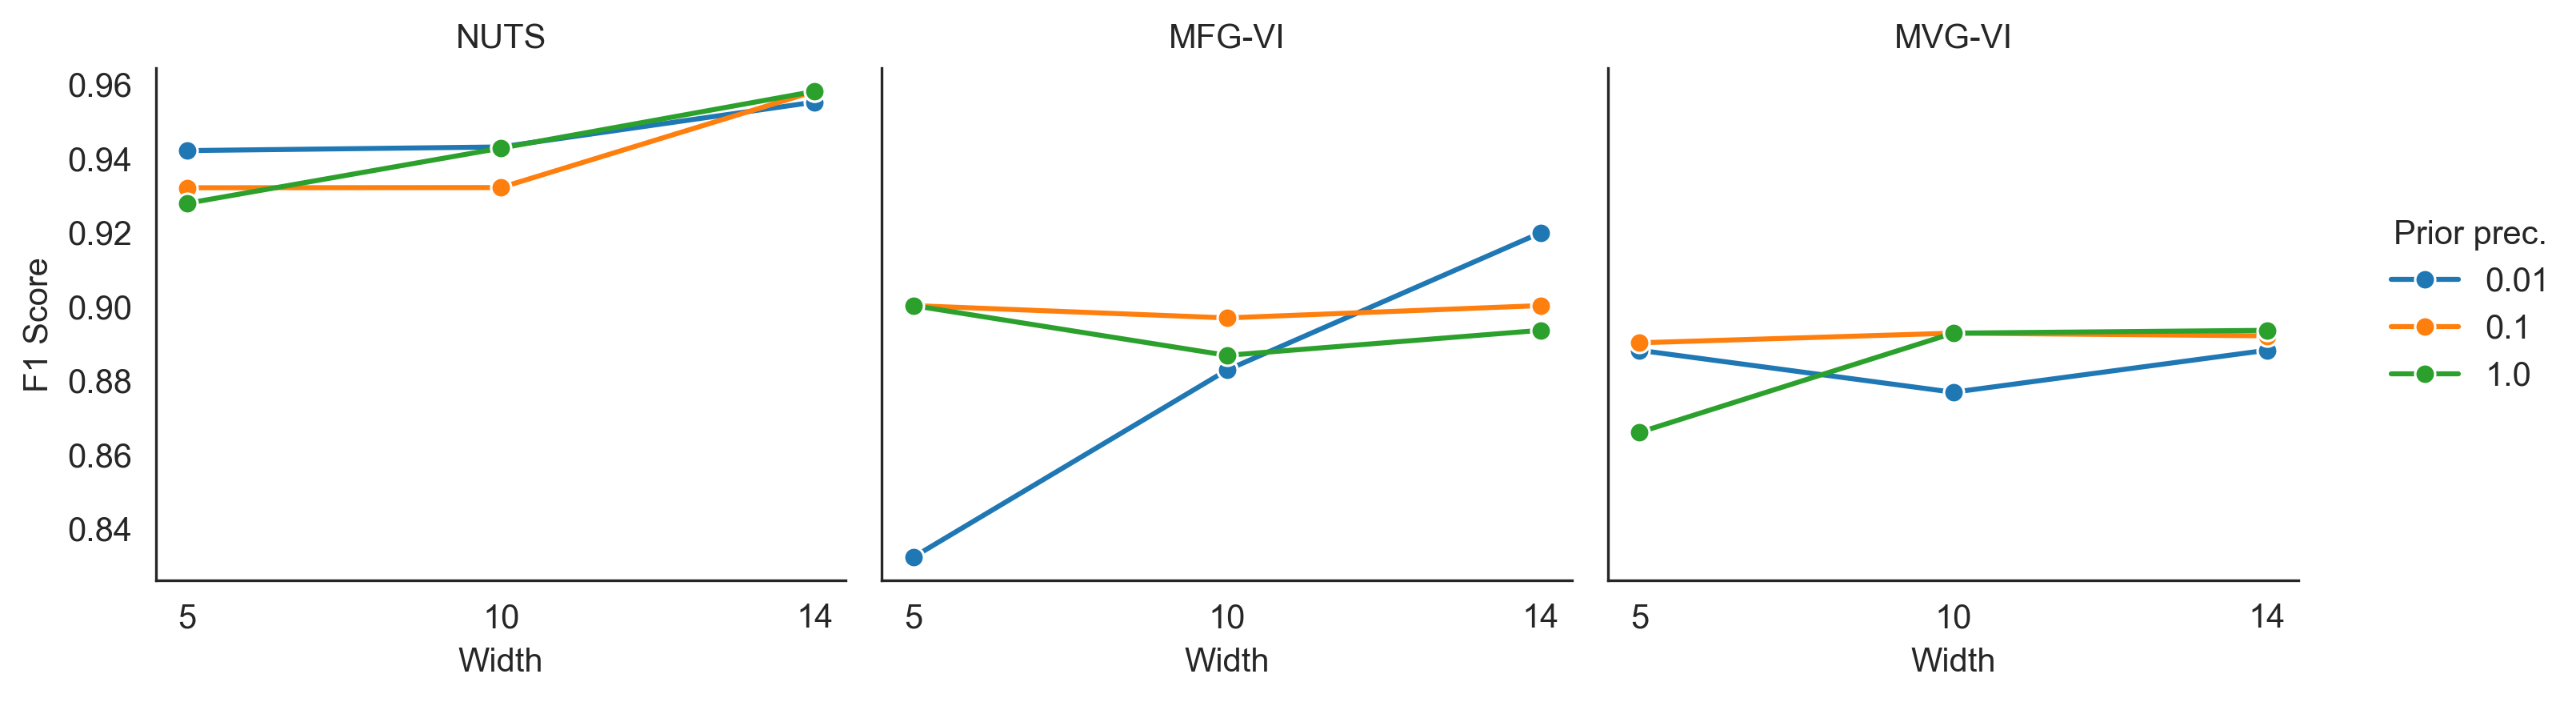
\includegraphics[keepaspectratio]{figures/f1_width_cat_precisionprior_by_method.png}}

}

\caption{\label{fig-f1}\(F_1\) scores across hidden layer widths and
prior precisions for each inference method.}

\end{figure}%

Figure~\ref{fig-f1} shows \(F_1\) scores by hidden layer width and prior
precision for each inference method. Overall, scale factor had little
effect on performance, except for the MFG-VI BNN with width 5 and prior
precision 0.01, which had a lower \(F_1\). This suggests models could
update prior beliefs from the data, yielding similar posteriors across
settings. Increasing hidden layer width provided minimal gains: NUTS
models showed a slight upward trend, while VI models showed no clear
improvement, except for the MFG-VI BNN with prior precision 0.01, which
improved substantially with width.

\begin{figure}

\centering{

\pandocbounded{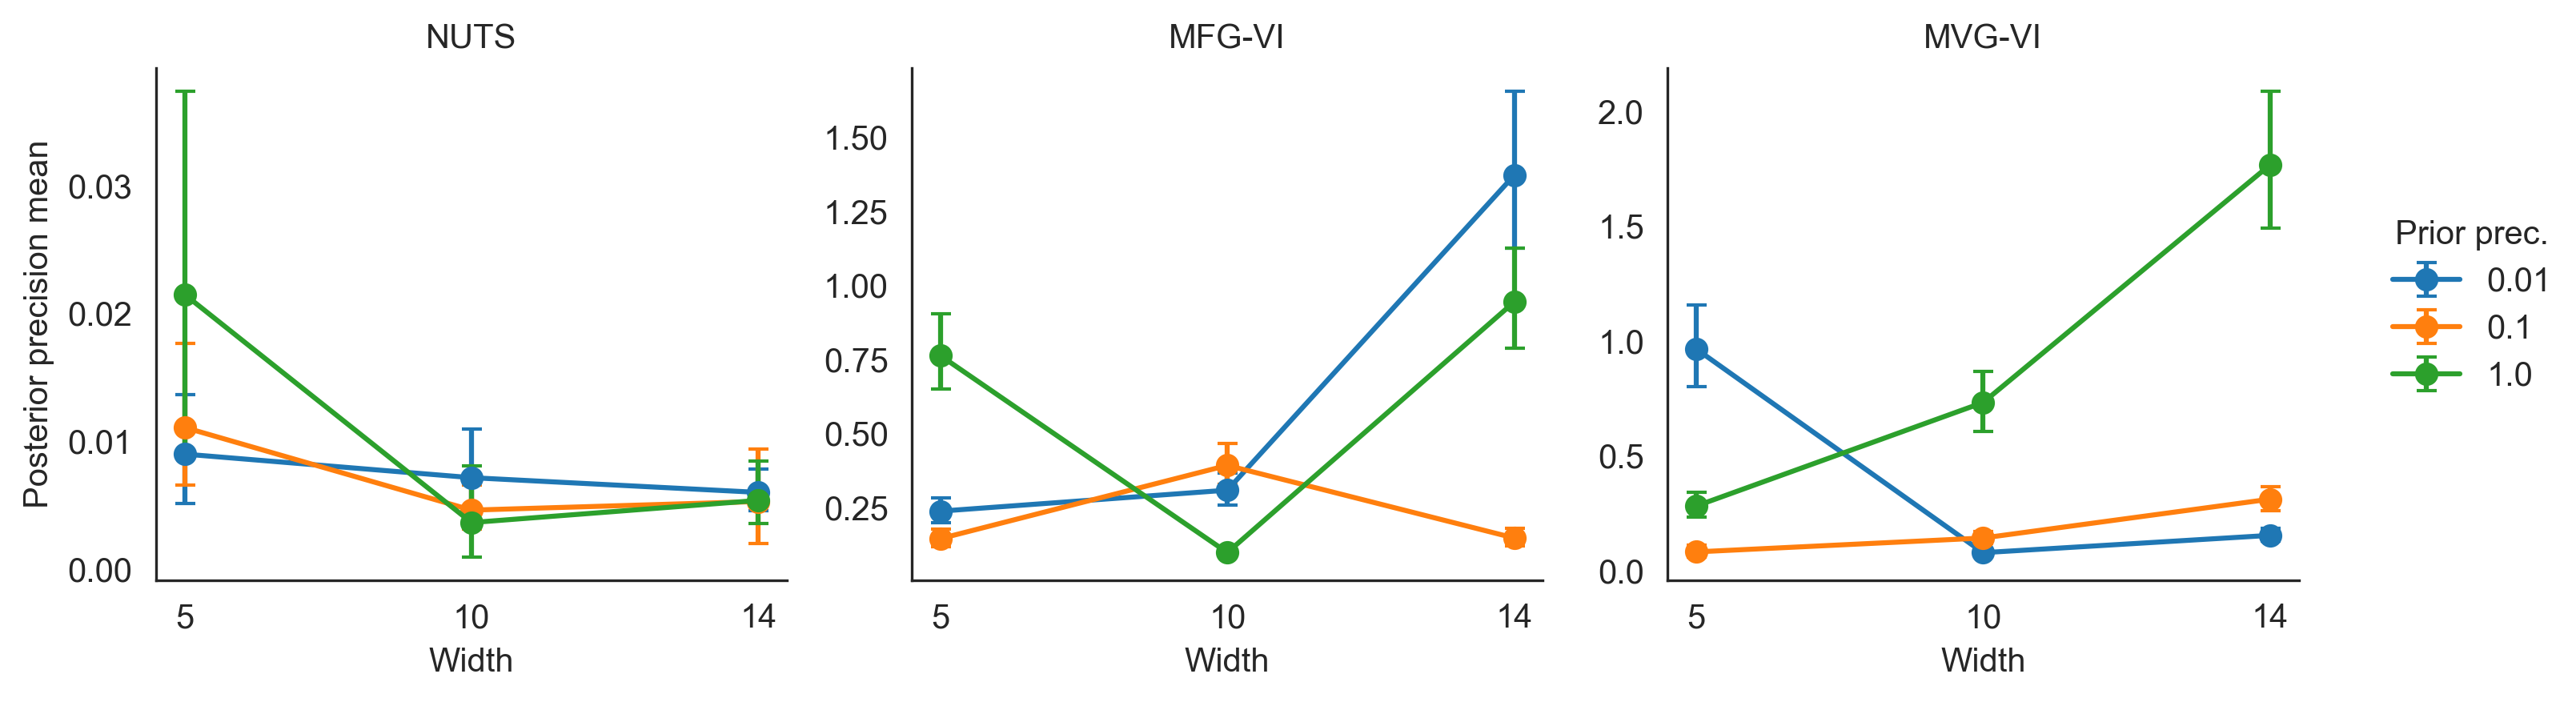
\includegraphics[keepaspectratio]{figures/precision_post_mean_ci_by_method.png}}

}

\caption{\label{fig-posterior}Posterior means and 95\% credible
intervals of the precision parameter by hidden layer width and prior
precision for each inference method.}

\end{figure}%

To examine prior precision effects, Figure~\ref{fig-posterior} shows
posterior means and 95\% CIs for the precision parameter by hidden layer
width and prior precision. NUTS-trained models with priors of 0.1 and 1
shifted toward \textasciitilde0.01, indicating increased parameter
variance, while models with a prior of 0.01 showed little change, with
narrower CIs at larger widths. VI-trained models moved toward
lower-variance parameters, with posterior means generally higher than
NUTS and no consistent trend in width. Notably, a prior precision of 0.1
tended to produce more precise (narrower) posterior estimates for the
precision parameter.

\begin{figure}

\centering{

\pandocbounded{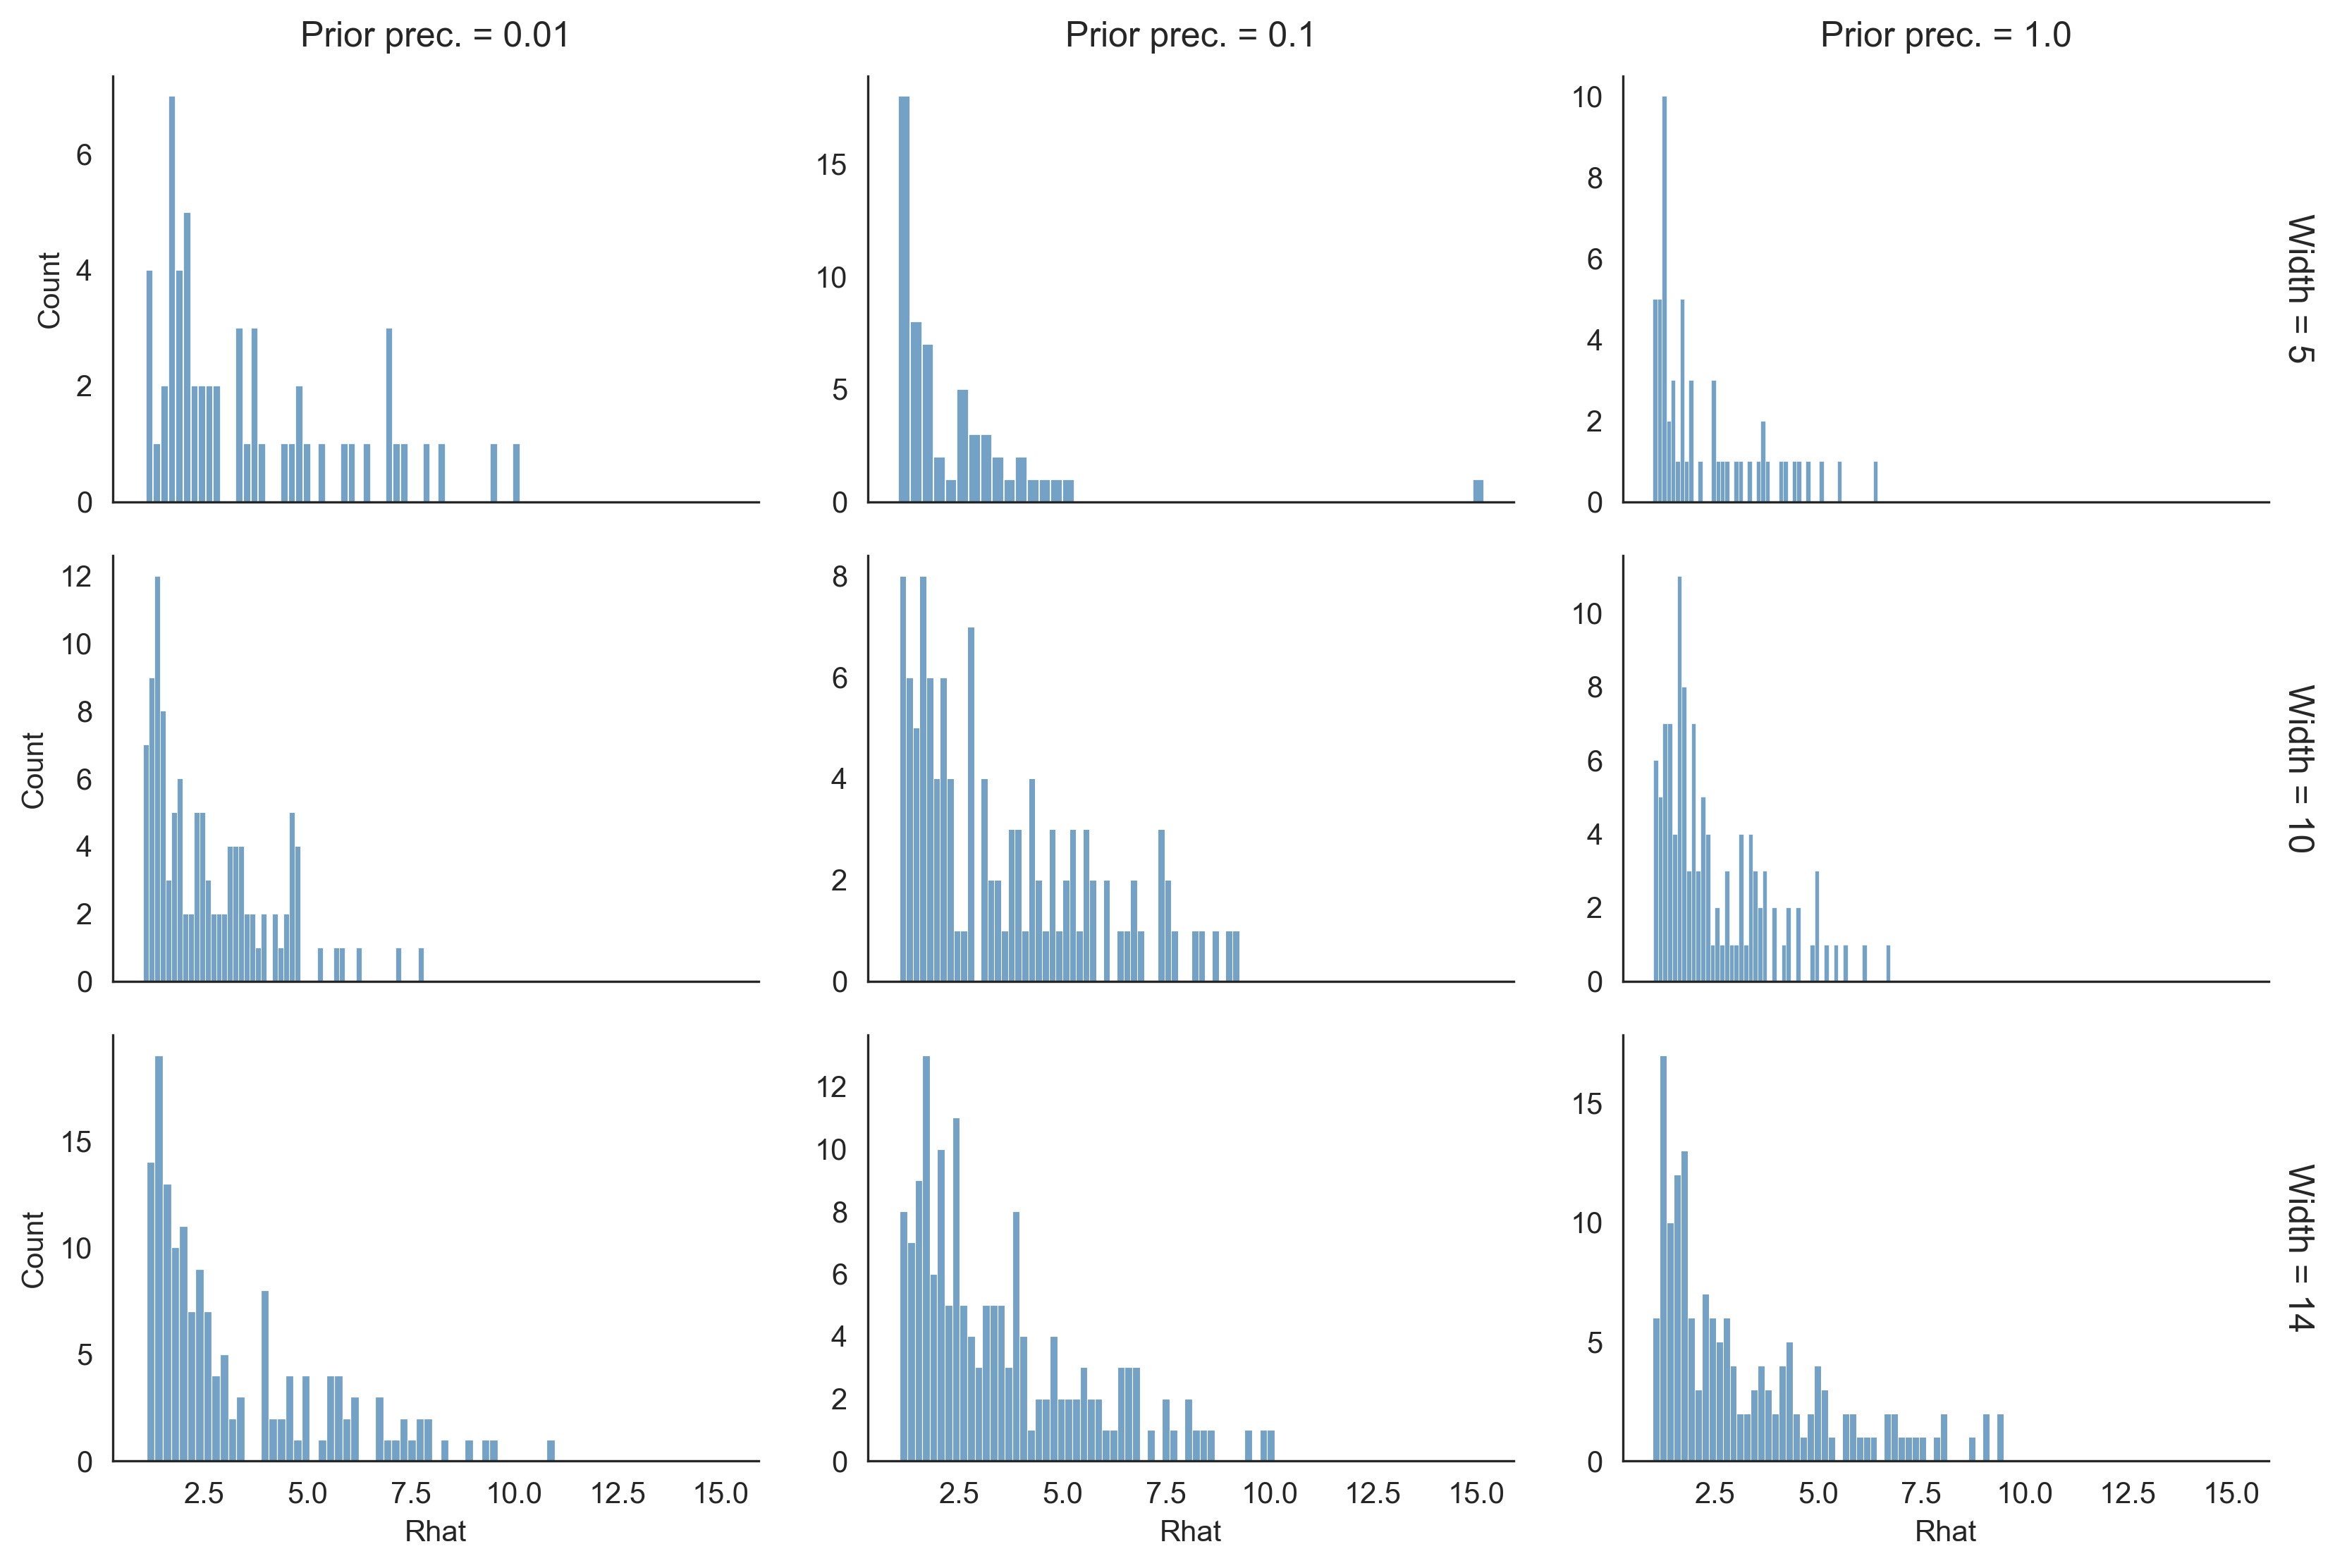
\includegraphics[keepaspectratio]{figures/rhat_histograms.png}}

}

\caption{\label{fig-rhat}Histograms of the \(\hat{R}\) statistic for
models trained with NUTS by hidden layer width and prior precision.}

\end{figure}%

Histograms of the \(\hat{R}\) statistic for NUTS-trained models are
shown in Figure~\ref{fig-rhat}. Most values cluster near 1, indicating
convergence, but some reach 10--15, signalling serious issues. ESS
histograms in Figure~\ref{fig-ess} confirm many parameters have
near-zero effective samples. Such results are expected for
high-dimensional BNNs (14) and could be mitigated with longer chains,
hyperparameter tuning, or thinning, but these approaches can be
computationally prohibitive.

\begin{figure}

\centering{

\pandocbounded{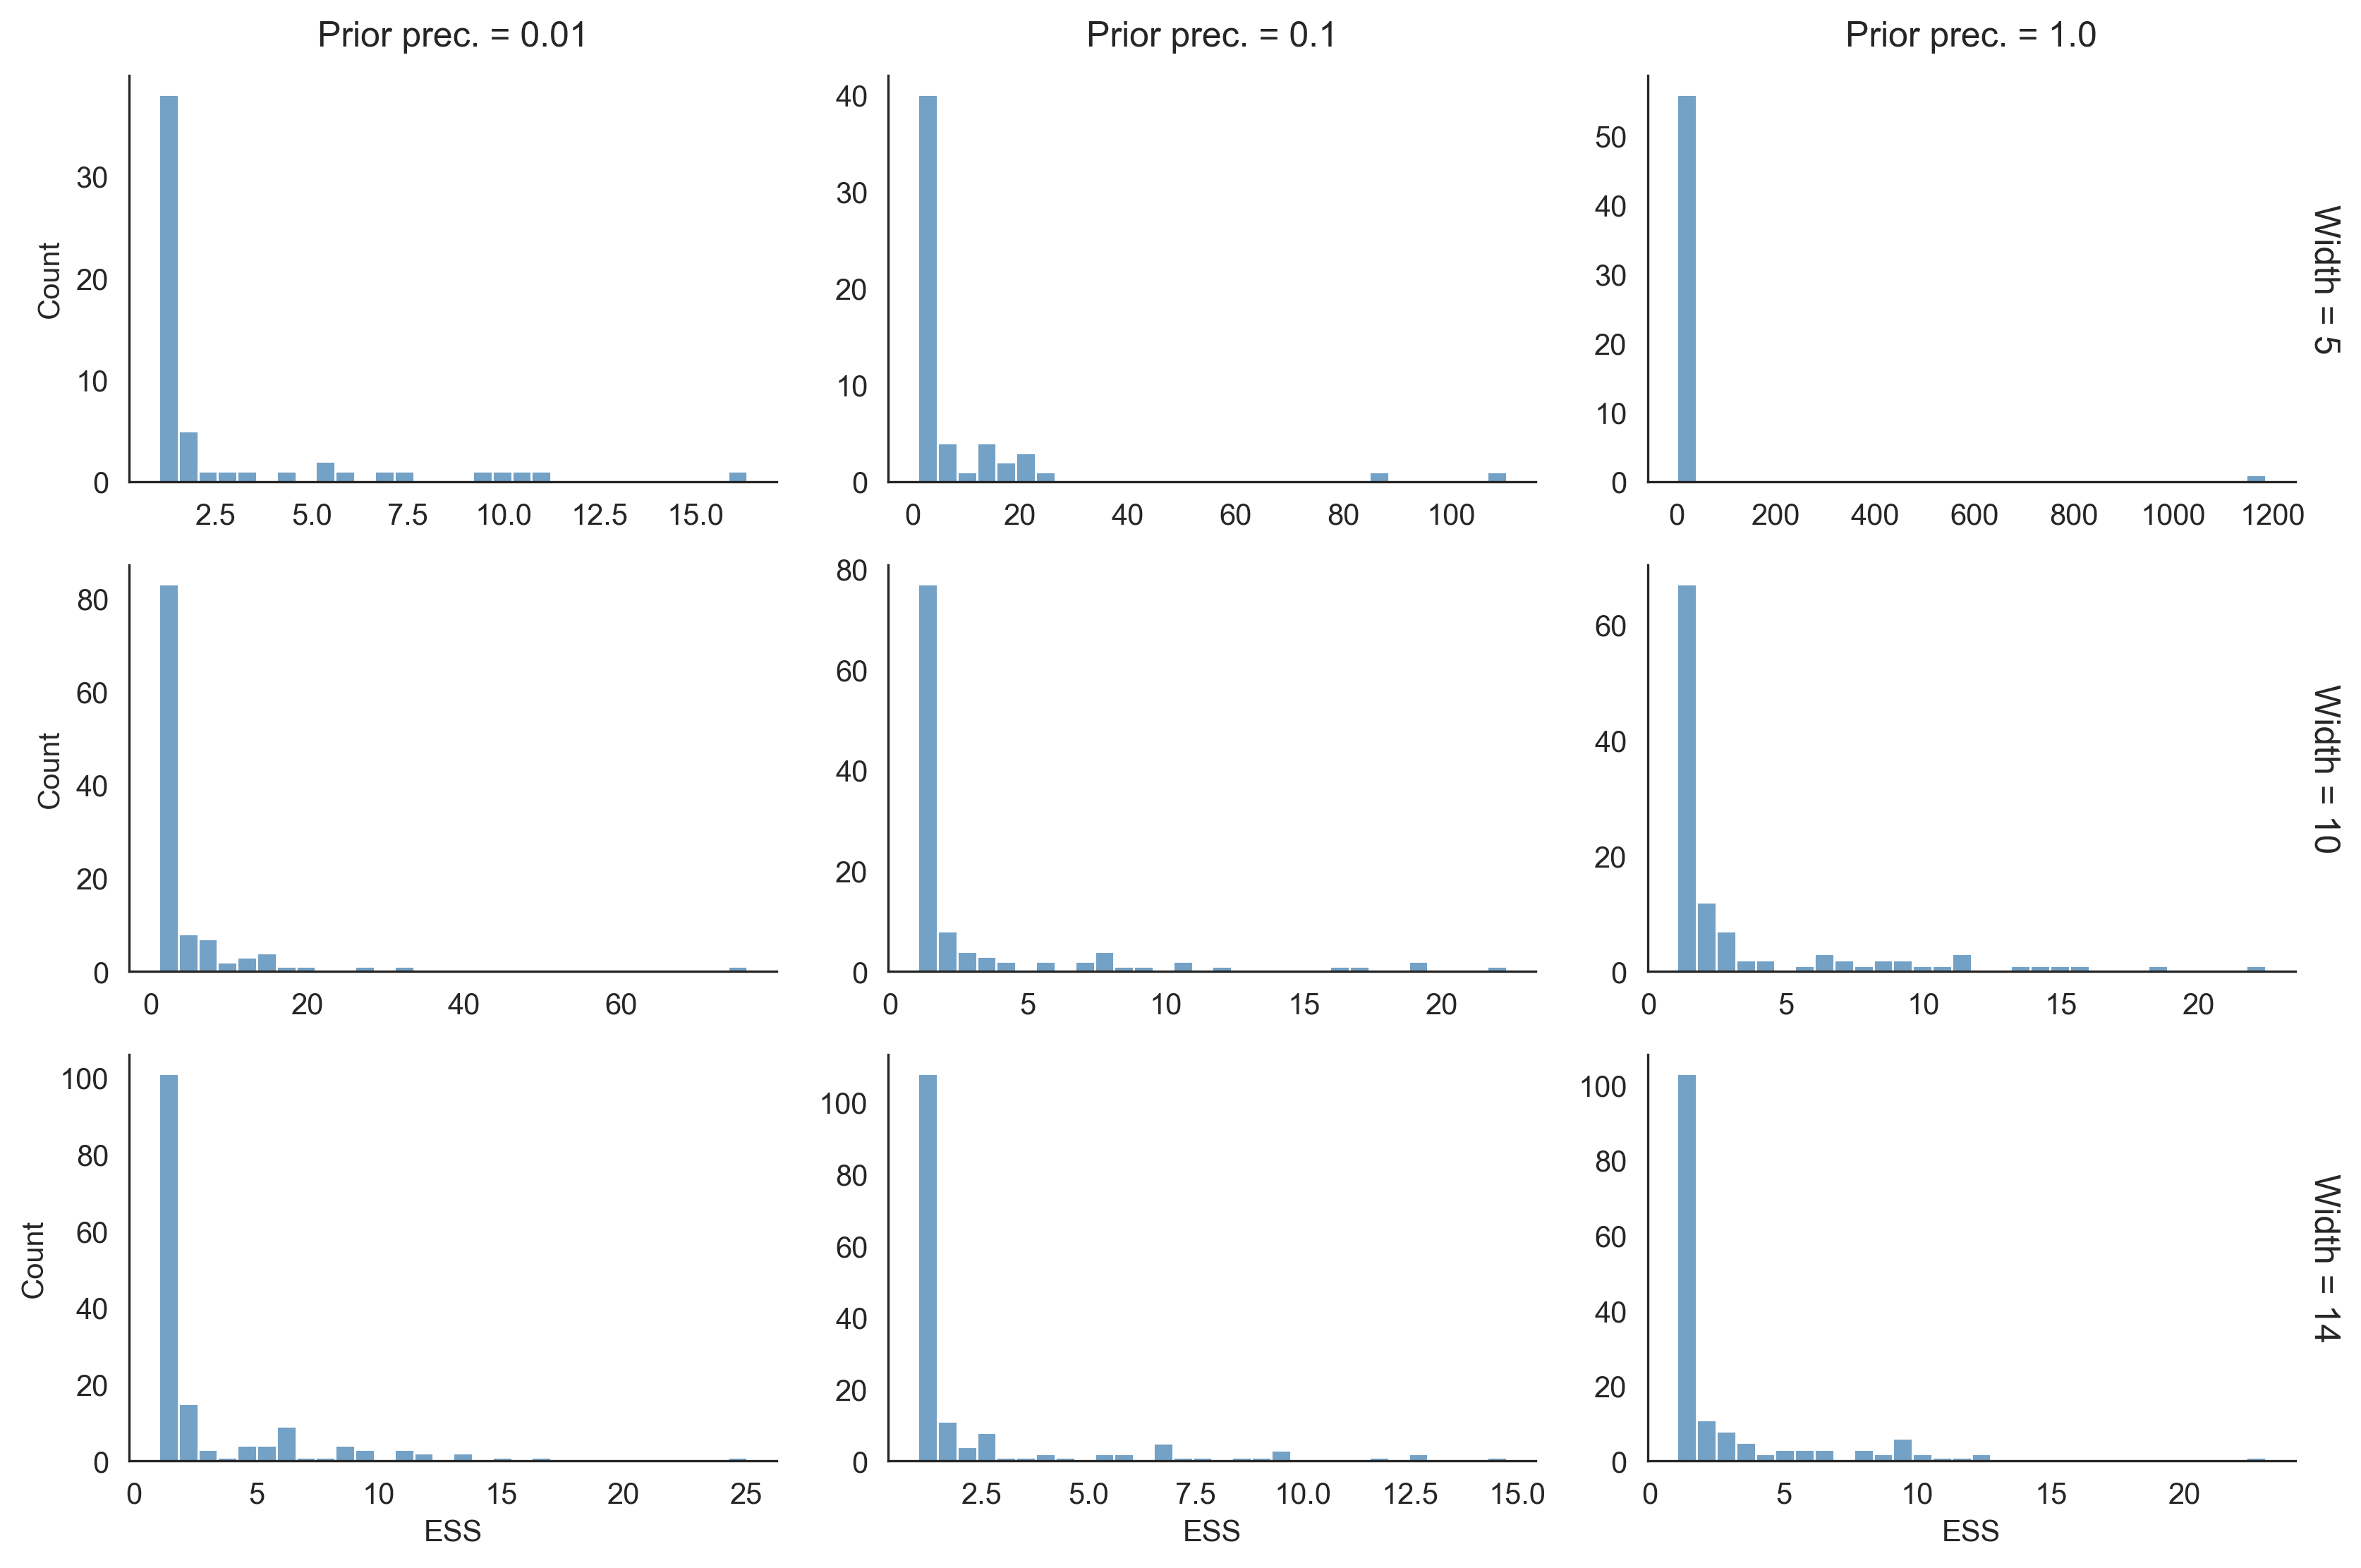
\includegraphics[keepaspectratio]{figures/ess_histograms.png}}

}

\caption{\label{fig-ess}Histograms of effective sample sizes (ESS) for
models trained with NUTS by hidden layer width and prior precision.}

\end{figure}%

Negative ELBO trace plots for VI models are shown in
Figure~\ref{fig-elbo}. Values plateau around iteration 1,000 and remain
stable by the end. MVG-VI models start with lower negative ELBOs than
MFG-VI, suggesting more efficient posterior approximation, but both
guides reach similar final values. However, comparable ELBOs do not
guarantee high-quality approximations, as VI can suffer from mode
collapse and guide flexibility is limited. These guides were chosen for
demonstration; more expressive families could improve performance in
practice.

\begin{figure}

\centering{

\pandocbounded{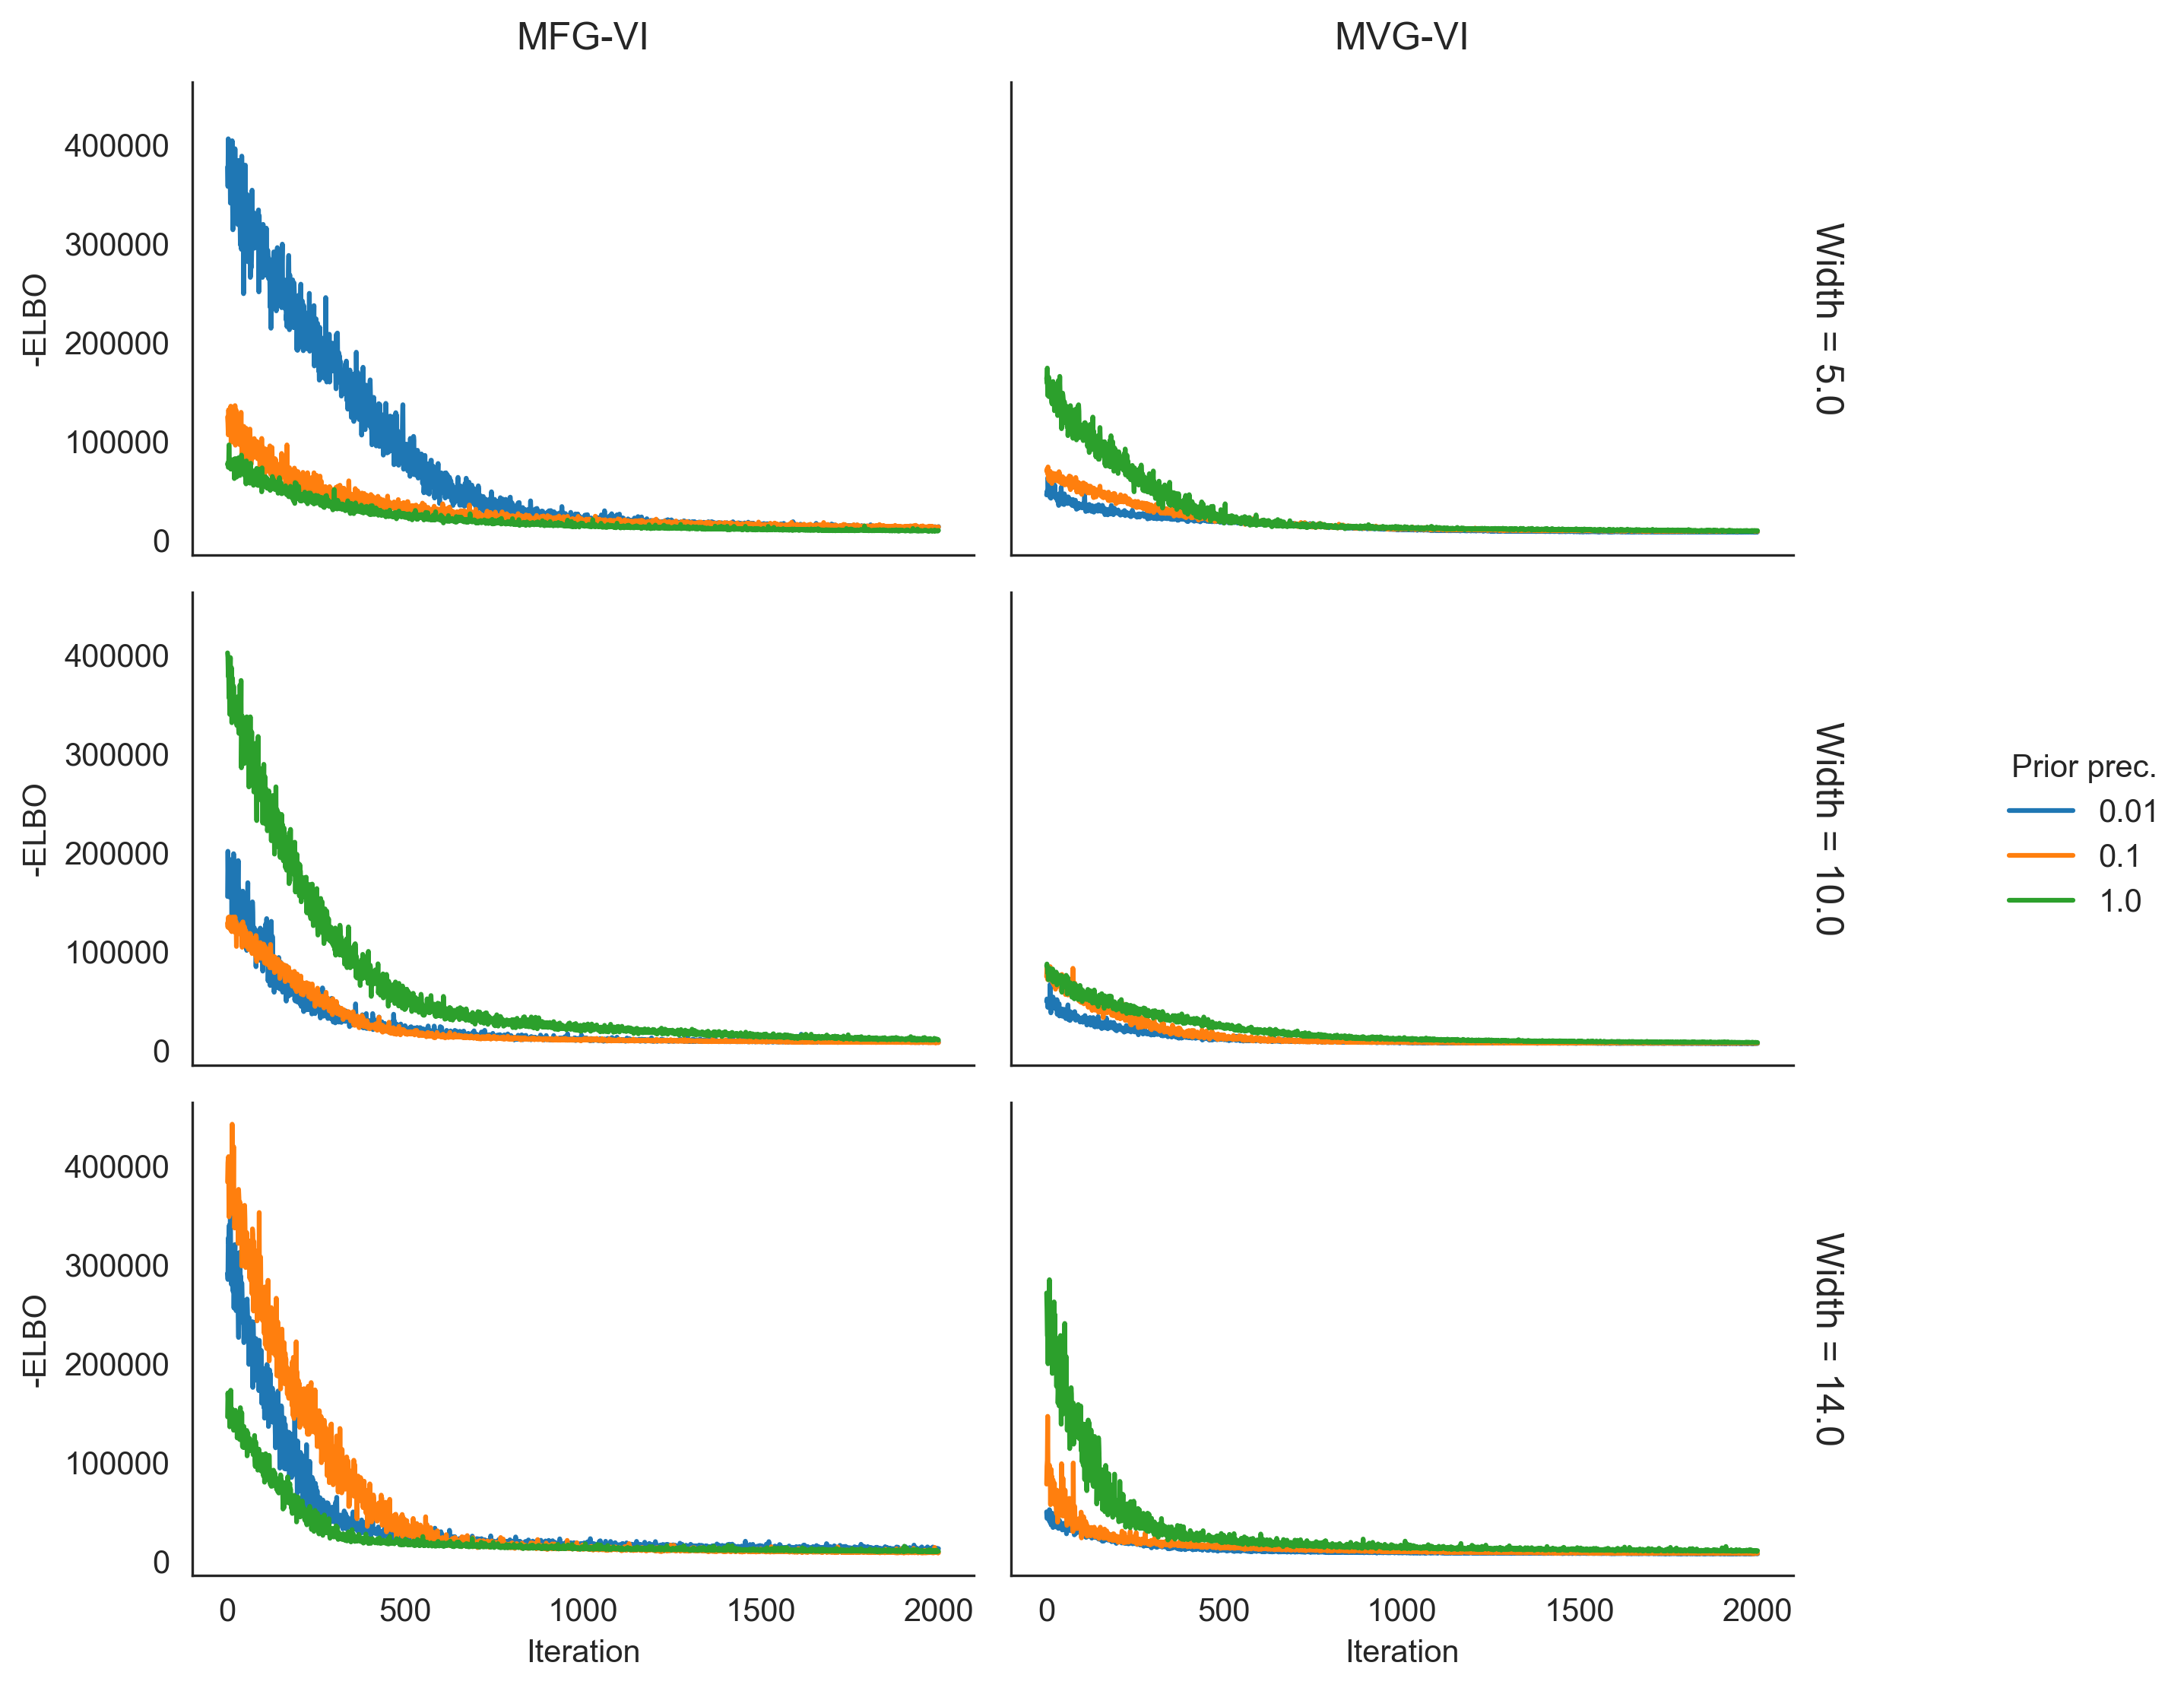
\includegraphics[keepaspectratio]{figures/elbo_traces_by_method_width.png}}

}

\caption{\label{fig-elbo}ELBO traces for VI-trained BNNs across
different hidden layer widths and prior precision levels.}

\end{figure}%

The best-performing BNN classifier on the validation data had a hidden
layer width of 14, a prior precision of 0.1, and was trained using NUTS,
achieving an \(F_1\) score of 0.958. Its prediction performance and
calibration quality on the test set were compared with those of a neural
network (NN) with the same hidden layer width and precision for
parameter initialisation, a gradient boosting decision tree (GBDT)
classifier, and calibrated versions of both the NN and GBDT classifiers.
The results are shown in Figure~\ref{fig-benchmarking}. Alongside
\(F_1\) scores, precision and recall values are also reported.

\begin{figure}

\centering{

\pandocbounded{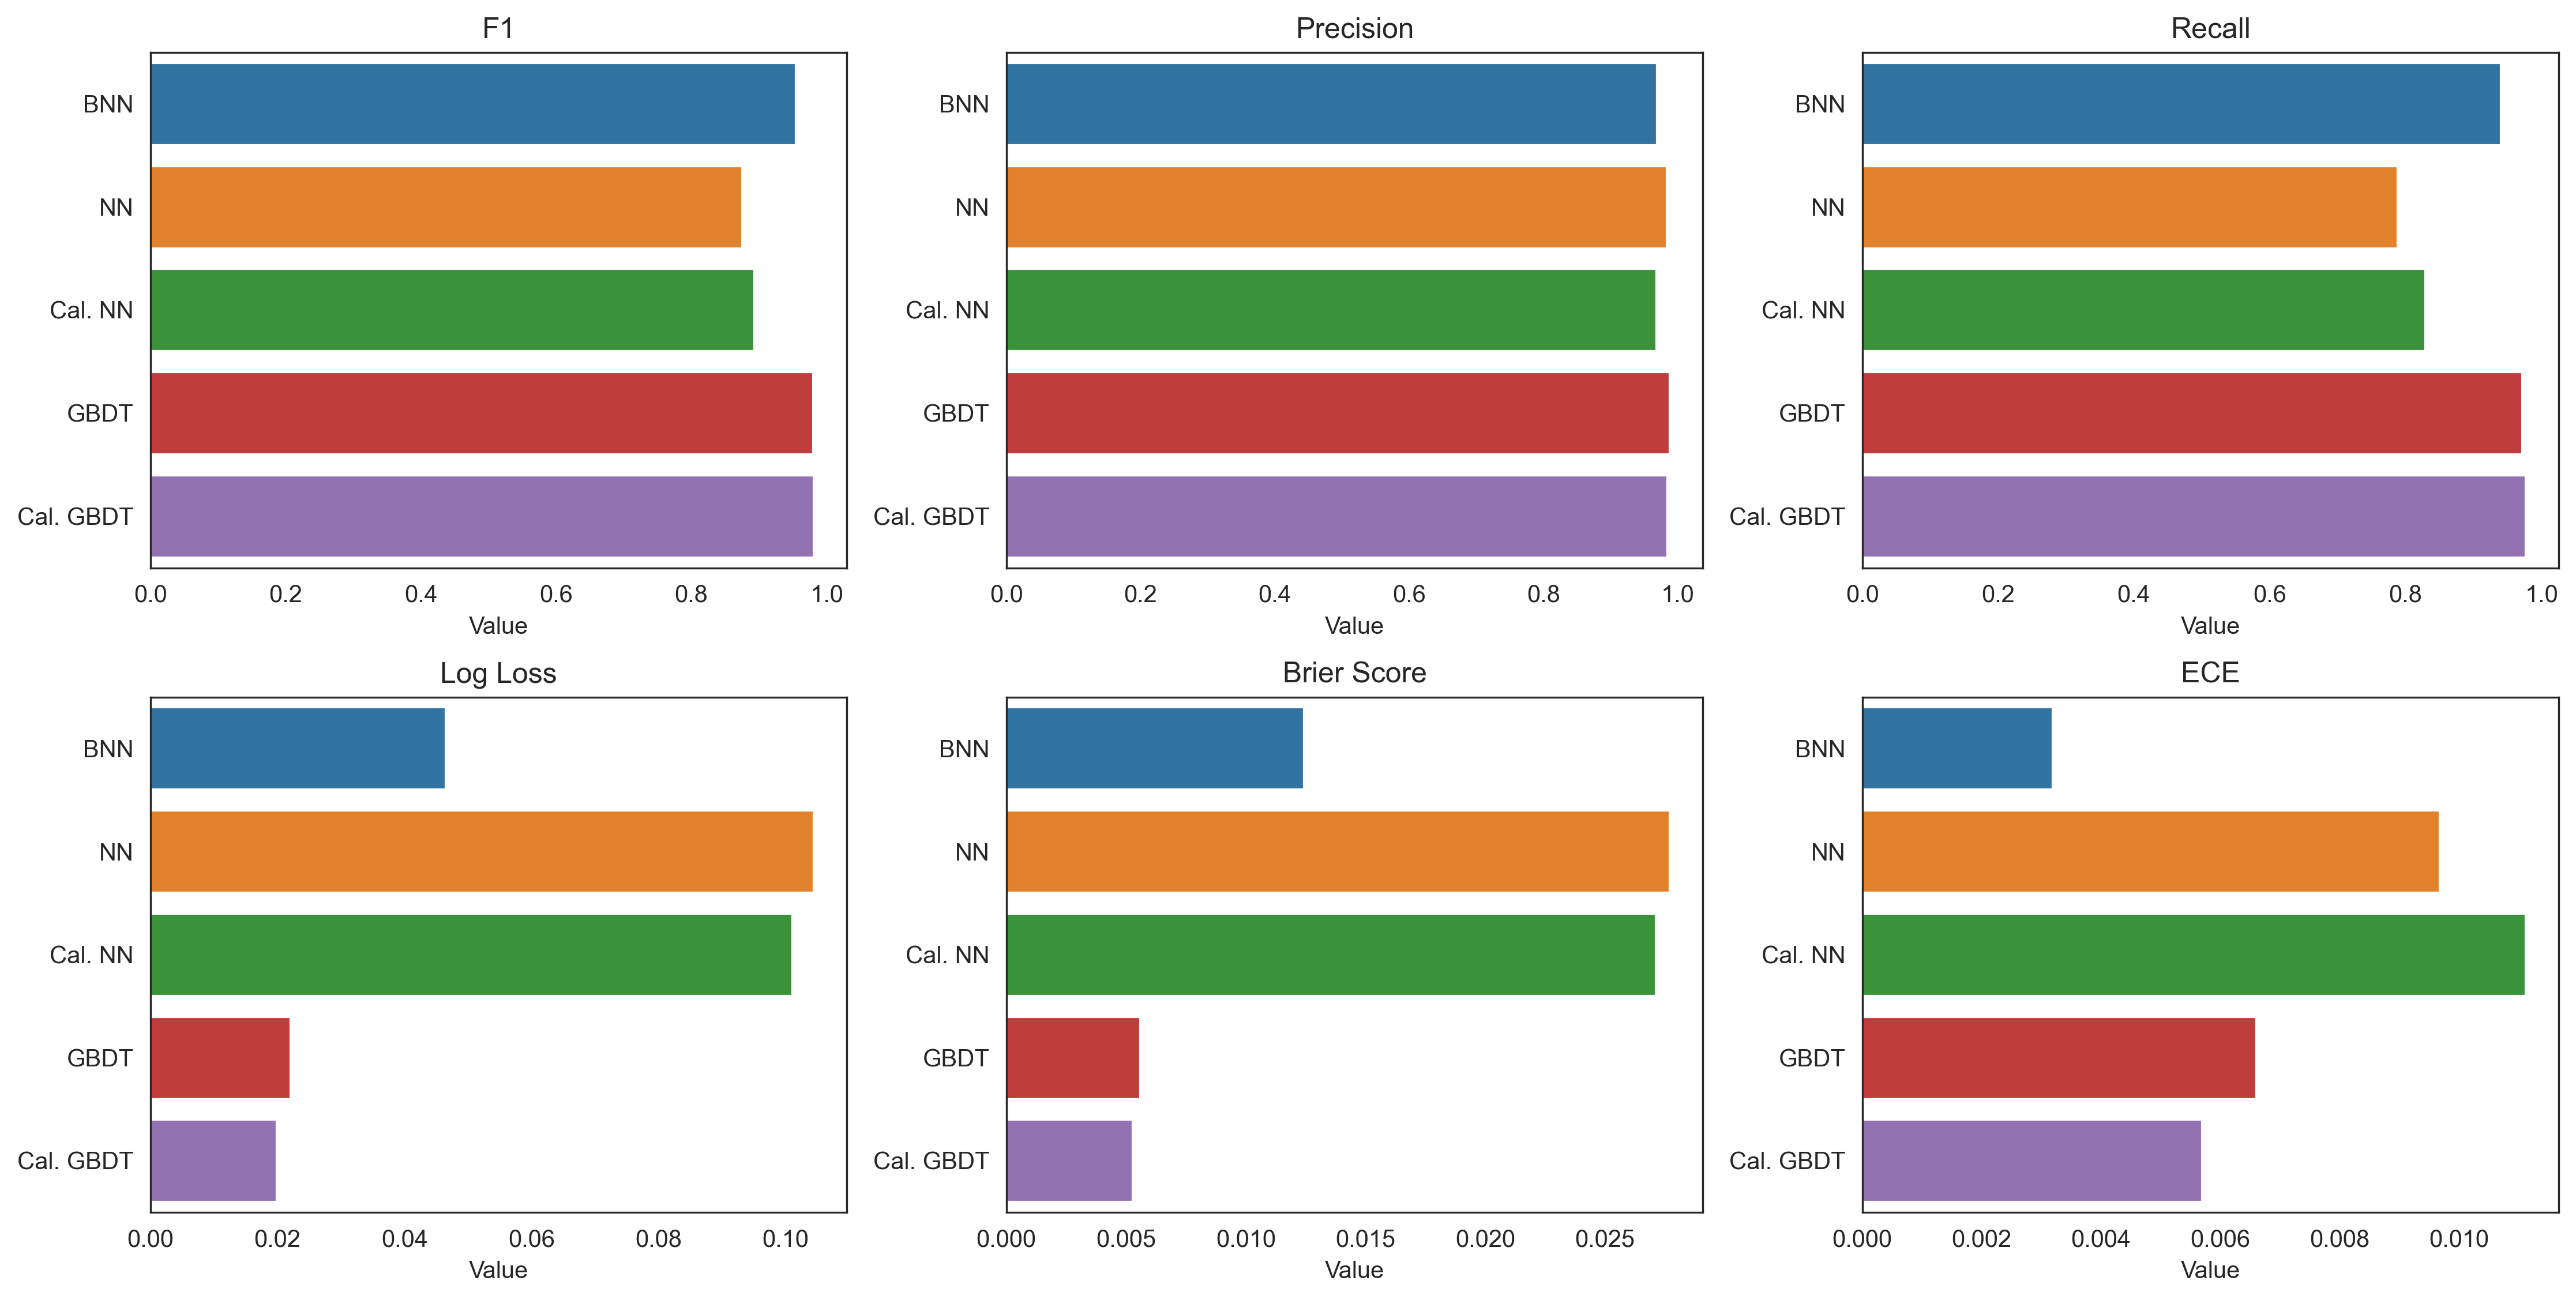
\includegraphics[keepaspectratio]{figures/benchmarking.png}}

}

\caption{\label{fig-benchmarking}Test set performance of all
classifiers, showing \(F_1\), precision, recall, log loss, Brier score,
and expected calibration error (ECE).}

\end{figure}%

Overall, all classifiers performed very well on the test set, with
prediction metrics close to 1. The BNN achieved a very close test
\(F_1\) score to the GBDT and calibrated GBDT classifiers, the
best-performing models, whereas the NN and calibrated NN scored slightly
lower. Precision was similar across all models, but recall was
noticeably lower for the NN and calibrated NN. For calibration metrics,
the NN and calibrated NN performed substantially worse than the other
models, with calibration improving only marginally and, in the case of
the expected calibration error (ECE), even worsening. In terms of log
loss, the GBDT classifiers achieved the lowest values, followed by the
BNN, with a similar pattern observed for the Brier score. The BNN
outperformed the GBDT models only on the ECE metric.

\begin{figure}

\centering{

\pandocbounded{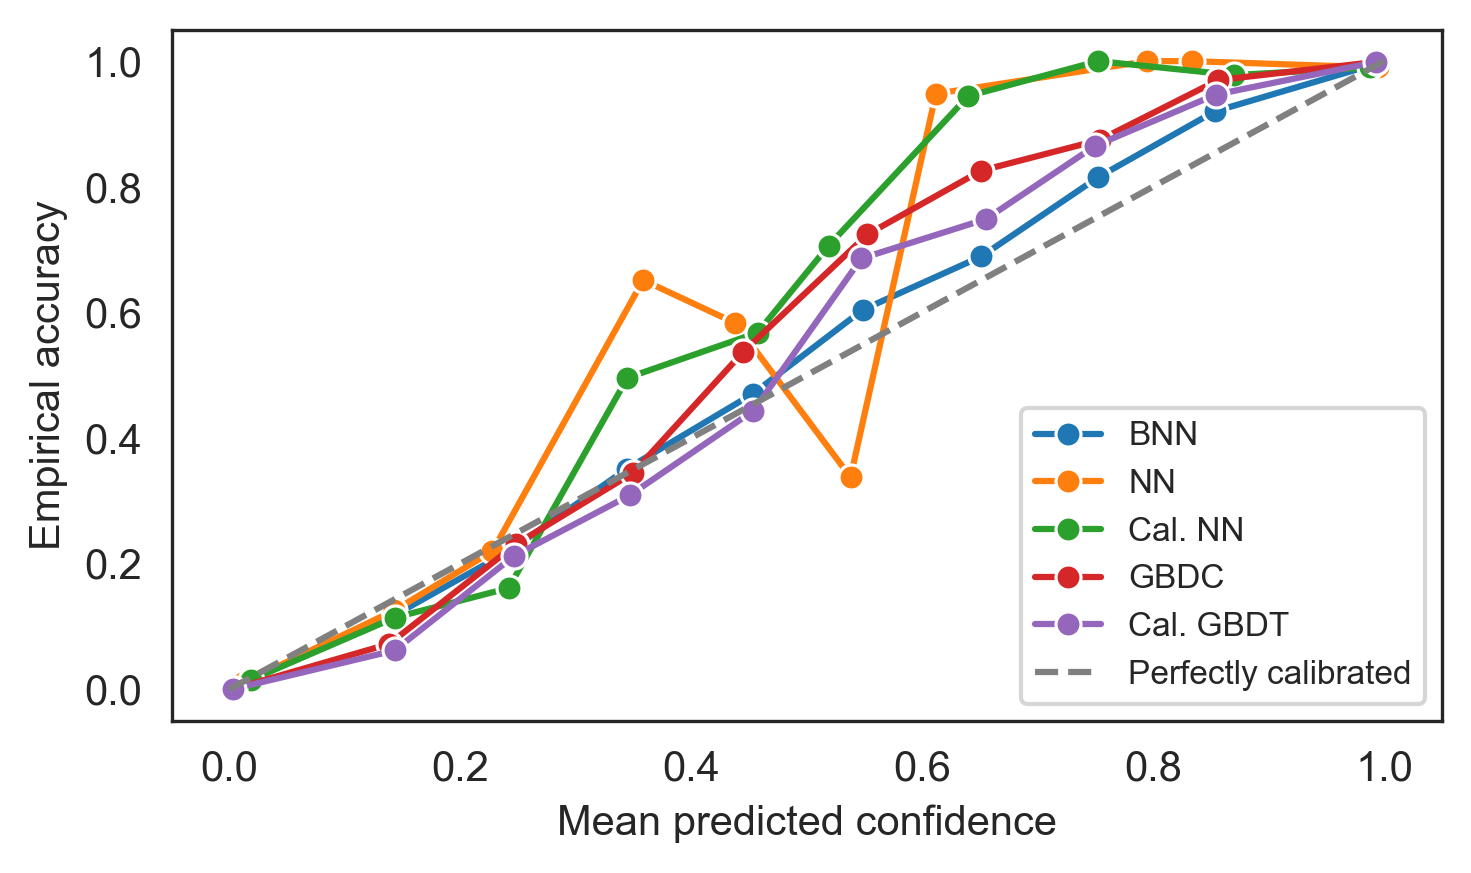
\includegraphics[keepaspectratio]{figures/calibration_curves.png}}

}

\caption{\label{fig-calibration}Test set calibration curves for all
benchmarked models.}

\end{figure}%

Calibration curves on the test set for the benchmarked models are shown
in Figure~\ref{fig-calibration}. The BNN's curve is the closest to the
identity line, indicating the best calibration among the models, which
is consistent with its lowest ECE value. In contrast, the NN and
calibrated NN curves deviate the most from the identity line, matching
their highest ECE values. Additionally, histograms of the predicted
probabilities on the test set are shown in Figure~\ref{fig-pred-probs}.
Concentrations of probabilities near 0 or 1 indicate high classifier
confidence. This pattern is evident for the BNN, GBDT, and calibrated
GBDT, whereas the NN and calibrated NN produce a larger proportion of
intermediate probabilities, suggesting lower confidence for some test
samples.

\begin{figure}

\centering{

\pandocbounded{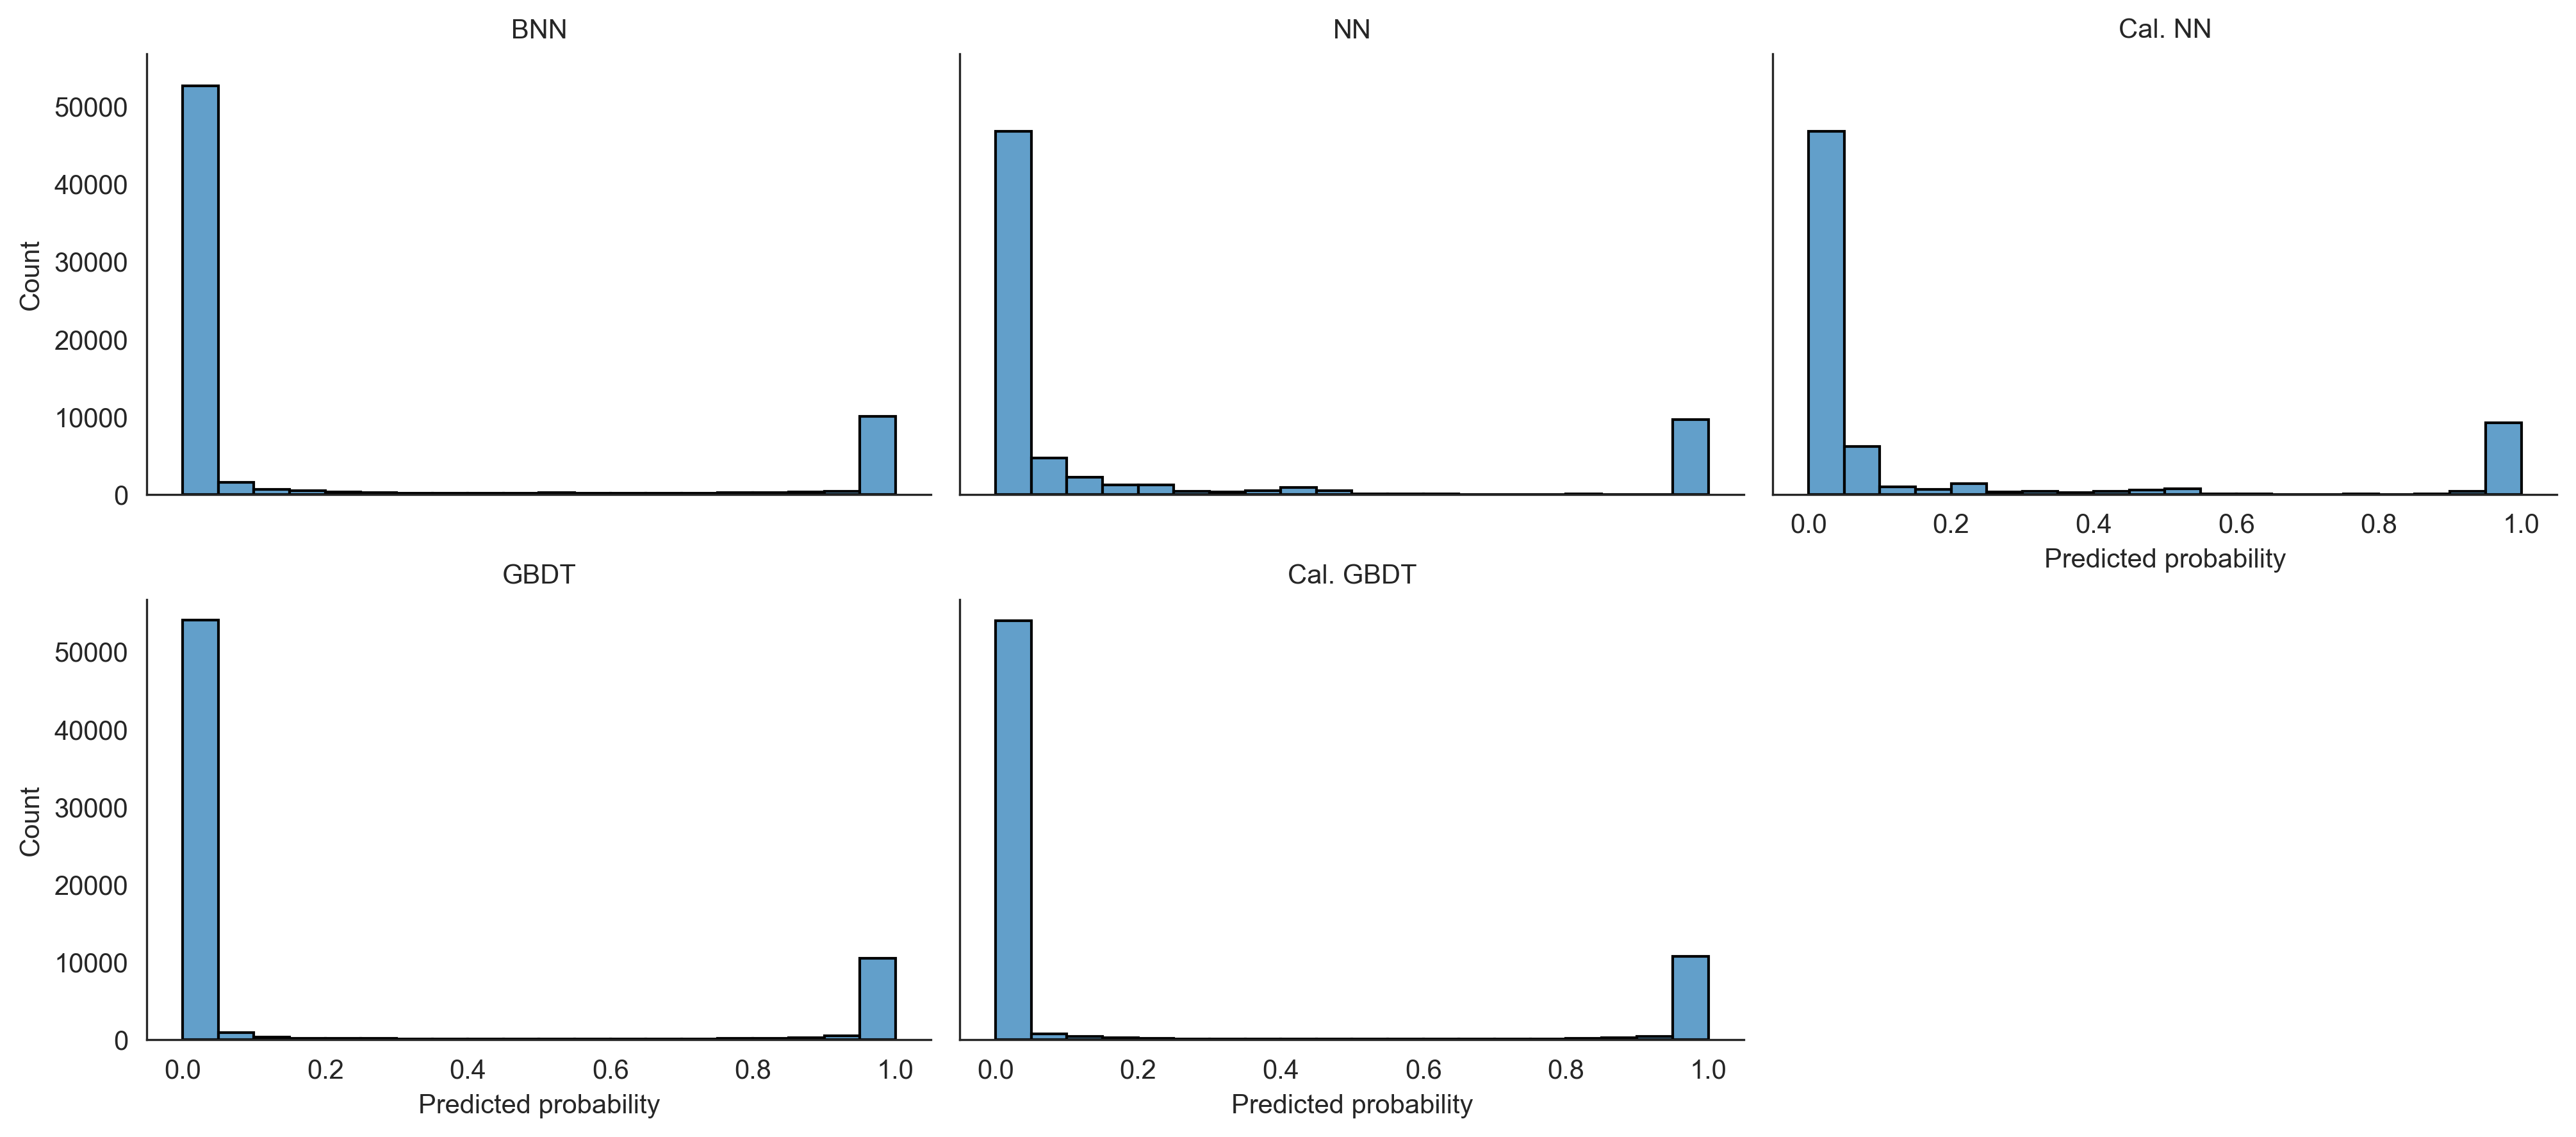
\includegraphics[keepaspectratio]{figures/pred_probs_hist.png}}

}

\caption{\label{fig-pred-probs}Histograms of predicted probabilities on
the test set for all benchmarked models.}

\end{figure}%

\bookmarksetup{startatroot}

\chapter{Conclusions}\label{conclusions}

In this study, we evaluated Bayesian Neural Networks (BNNs) for
cyber-attack detection using the UNSW-NB15 dataset. The analysis focused
on two main objectives: (i) assessing different BNN configurations
relevant for real-world deployment, including inference method, model
architecture complexity, and prior specification, and (ii) benchmarking
BNNs against high-performing models for tabular classification tasks.

We found that Markov Chain Monte Carlo (MCMC), specifically the
No-U-Turn Sampler (NUTS), consistently outperformed variational
inference (VI) methods in predictive performance. This is likely due to
MCMC's ability to generate samples from the true posterior under
convergence, whereas VI methods approximate the posterior with simpler
distributions that require careful tuning. However, MCMC was
computationally expensive, taking roughly 100 times longer to train than
VI, which completed in seconds. While VI is more scalable, the
restrictive variational distributions used in this study limited
performance. Future applications should explore more flexible
approximations to improve accuracy. Model complexity, measured by the
width of the hidden layer, and prior specification, defined as the
precision prior, had no substantial impact on results.

The best-performing BNN, trained with MCMC, achieved predictive
performance comparable to gradient boosted decision trees (GBDTs), which
are a common benchmark for classification. In terms of calibration,
although GBDTs generally outperformed the BNN except in expected
calibration error (ECE), the BNN still provided a marked improvement
over a non-Bayesian neural network (NN). These findings indicate that
BNNs can be competitive for classification while offering the additional
advantage of quantifying predictive uncertainty, which GBDTs and
frequentist NNs cannot provide.

Unexpectedly, the MCMC algorithm did not fully converge to the posterior
distribution and was in fact far from convergence, yet still delivered
competitive results. This suggests that, in this setting, full
convergence may not be strictly necessary for strong predictive
performance, particularly if the data exert a strong influence on the
learned parameter distributions.

Lastly, the strong performance on this moderately imbalanced dataset,
without any balancing techniques, suggests a strong signal for
identifying cyber-attacks, possibly due to the dataset being
artificially generated. These results may not generalise to real-world
data, where handling class imbalance could be necessary before deploying
BNNs or other models.

\bookmarksetup{startatroot}

\chapter*{Generative AI
Acknowledgment}\label{generative-ai-acknowledgment}
\addcontentsline{toc}{chapter}{Generative AI Acknowledgment}

\markboth{Generative AI Acknowledgment}{Generative AI Acknowledgment}

\begin{itemize}
\item
  I acknowledge the use of ChatGPT-4o (\url{https://chatgpt.com/}) to
  identify improvements in the writing style.
\item
  I acknowledge the use of ChatGPT-4o (\url{https://chatgpt.com/}) to
  aid my understanding of concepts and to validate the technical
  accuracy of my ideas for data analysis.
\item
  I acknowledge the use of ChatGPT-4o (\url{https://chatgpt.com/}) to
  create snippets of code for debugging and data analysis.
\end{itemize}

\bookmarksetup{startatroot}

\chapter*{References}\label{references}
\addcontentsline{toc}{chapter}{References}

\markboth{References}{References}

\phantomsection\label{refs}
\begin{CSLReferences}{0}{1}
\bibitem[\citeproctext]{ref-moustafa2015unsw}
\CSLLeftMargin{1. }%
\CSLRightInline{Moustafa N, Slay J. UNSW-NB15: A comprehensive data set
for network intrusion detection systems (UNSW-NB15 network data set).
In: 2015 military communications and information systems conference
(MilCIS). IEEE; 2015. p. 1--6. }

\bibitem[\citeproctext]{ref-moustafa2016evaluation}
\CSLLeftMargin{2. }%
\CSLRightInline{Moustafa N, Slay J. The evaluation of network anomaly
detection systems: Statistical analysis of the UNSW-NB15 data set and
the comparison with the KDD99 data set. Information Security Journal: A
Global Perspective. 2016;25(1-3):18--31. }

\bibitem[\citeproctext]{ref-zoghi2021unsw}
\CSLLeftMargin{3. }%
\CSLRightInline{Zoghi Z, Serpen G. UNSW-NB15 computer security dataset:
Analysis through visualization. arXiv preprint arXiv:210105067. 2021; }

\bibitem[\citeproctext]{ref-unsw2015nb15}
\CSLLeftMargin{4. }%
\CSLRightInline{University of New South Wales (UNSW). UNSW-NB15 dataset
{[}Internet{]}. 2015. Available from:
\url{https://research.unsw.edu.au/projects/unsw-nb15-dataset}}

\bibitem[\citeproctext]{ref-ttl}
\CSLLeftMargin{5. }%
\CSLRightInline{Imperva. Time to live (TTL) {[}Internet{]}. n.d.
Available from:
\url{https://www.imperva.com/learn/performance/time-to-live-ttl/}}

\bibitem[\citeproctext]{ref-hyndman2013transformations}
\CSLLeftMargin{6. }%
\CSLRightInline{Hyndman RJ. Transforming data with zeros {[}Internet{]}.
2013. Available from:
\url{https://robjhyndman.com/hyndsight/transformations/}}

\bibitem[\citeproctext]{ref-ross2014mutual}
\CSLLeftMargin{7. }%
\CSLRightInline{Ross BC. Mutual information between discrete and
continuous data sets. PloS one. 2014;9(2):e87357. }

\bibitem[\citeproctext]{ref-sklearn-mi}
\CSLLeftMargin{8. }%
\CSLRightInline{scikit‑learn Developers. Scikit\-learn:
mutual\_info\_classif.
\url{https://scikit-learn.org/stable/modules/generated/sklearn.feature_selection.mutual_info_classif.html};
2025. }

\bibitem[\citeproctext]{ref-sklearn-rfclassifier}
\CSLLeftMargin{9. }%
\CSLRightInline{scikit‑learn Developers. Scikit\-learn:
RandomForestClassifier.
\url{https://scikit-learn.org/stable/modules/generated/sklearn.ensemble.RandomForestClassifier.html};
2025. }

\bibitem[\citeproctext]{ref-arbel2023primer}
\CSLLeftMargin{10. }%
\CSLRightInline{Arbel J, Pitas K, Vladimirova M, Fortuin V. A primer on
bayesian neural networks: Review and debates. arXiv preprint
arXiv:230916314. 2023; }

\bibitem[\citeproctext]{ref-jospin2022hands}
\CSLLeftMargin{11. }%
\CSLRightInline{Jospin LV, Laga H, Boussaid F, Buntine W, Bennamoun M.
Hands-on bayesian neural networks---a tutorial for deep learning users.
IEEE Computational Intelligence Magazine. 2022;17(2):29--48. }

\bibitem[\citeproctext]{ref-adam2014method}
\CSLLeftMargin{12. }%
\CSLRightInline{Adam KDBJ et al. A method for stochastic optimization.
arXiv preprint arXiv:14126980. 2014;1412(6). }

\bibitem[\citeproctext]{ref-goodfellow2016deep}
\CSLLeftMargin{13. }%
\CSLRightInline{Goodfellow I, Bengio Y, Courville A, Bengio Y. Deep
learning. Vol. 1. MIT press Cambridge; 2016. }

\bibitem[\citeproctext]{ref-izmailov2021bayesian}
\CSLLeftMargin{14. }%
\CSLRightInline{Izmailov P, Vikram S, Hoffman MD, Wilson AGG. What are
bayesian neural network posteriors really like? In: International
conference on machine learning. PMLR; 2021. p. 4629--40. }

\bibitem[\citeproctext]{ref-wenzel2020good}
\CSLLeftMargin{15. }%
\CSLRightInline{Wenzel F, Roth K, Veeling BS, Świątkowski J, Tran L,
Mandt S, et al. How good is the bayes posterior in deep neural networks
really? arXiv preprint arXiv:200202405. 2020; }

\bibitem[\citeproctext]{ref-murphy2012machine}
\CSLLeftMargin{16. }%
\CSLRightInline{Murphy KP. Machine learning: A probabilistic
perspective. MIT press; 2012. }

\bibitem[\citeproctext]{ref-stan_ref}
\CSLLeftMargin{17. }%
\CSLRightInline{Stan Development Team. Stan reference manual version
2.36 {[}Internet{]}. 2024. Available from:
\url{https://mc-stan.org/docs/reference-manual/}}

\bibitem[\citeproctext]{ref-neal2011mcmc}
\CSLLeftMargin{18. }%
\CSLRightInline{Neal RM et al. MCMC using hamiltonian dynamics. Handbook
of markov chain monte carlo. 2011;2(11):2. }

\bibitem[\citeproctext]{ref-hoffman2014no}
\CSLLeftMargin{19. }%
\CSLRightInline{Hoffman MD, Gelman A, et al. The no-u-turn sampler:
Adaptively setting path lengths in hamiltonian monte carlo. J Mach Learn
Res. 2014;15(1):1593--623. }

\bibitem[\citeproctext]{ref-blei2017variational}
\CSLLeftMargin{20. }%
\CSLRightInline{Blei DM, Kucukelbir A, McAuliffe JD. Variational
inference: A review for statisticians. Journal of the American
statistical Association. 2017;112(518):859--77. }

\bibitem[\citeproctext]{ref-blundell2015weight}
\CSLLeftMargin{21. }%
\CSLRightInline{Blundell C, Cornebise J, Kavukcuoglu K, Wierstra D.
Weight uncertainty in neural network. In: International conference on
machine learning. PMLR; 2015. p. 1613--22. }

\bibitem[\citeproctext]{ref-hernandez2015probabilistic}
\CSLLeftMargin{22. }%
\CSLRightInline{Hernández-Lobato JM, Adams R. Probabilistic
backpropagation for scalable learning of bayesian neural networks. In:
International conference on machine learning. PMLR; 2015. p. 1861--9. }

\bibitem[\citeproctext]{ref-guo2017calibration}
\CSLLeftMargin{23. }%
\CSLRightInline{Guo C, Pleiss G, Sun Y, Weinberger KQ. On calibration of
modern neural networks. In: International conference on machine
learning. PMLR; 2017. p. 1321--30. }

\bibitem[\citeproctext]{ref-phan2019composable}
\CSLLeftMargin{24. }%
\CSLRightInline{Phan D, Pradhan N, Jankowiak M. Composable effects for
flexible and accelerated probabilistic programming in NumPyro. arXiv
preprint arXiv:191211554. 2019; }

\bibitem[\citeproctext]{ref-bingham2019pyro}
\CSLLeftMargin{25. }%
\CSLRightInline{Bingham E, Chen JP, Jankowiak M, Obermeyer F, Pradhan N,
Karaletsos T, et al. Pyro: Deep universal probabilistic programming. J
Mach Learn Res {[}Internet{]}. 2019;20:28:1--6. Available from:
\url{http://jmlr.org/papers/v20/18-403.html}}

\bibitem[\citeproctext]{ref-he2015delving}
\CSLLeftMargin{26. }%
\CSLRightInline{He K, Zhang X, Ren S, Sun J. Delving deep into
rectifiers: Surpassing human-level performance on imagenet
classification. In: Proceedings of the IEEE international conference on
computer vision. 2015. p. 1026--34. }

\bibitem[\citeproctext]{ref-scikit-learn-calibratedclass}
\CSLLeftMargin{27. }%
\CSLRightInline{scikit-learn Developers. Scikit\-learn:
CalibratedClassifierCV.
\url{https://scikit-learn.org/stable/modules/generated/sklearn.calibration.CalibratedClassifierCV.html};
2025. }

\bibitem[\citeproctext]{ref-scikit-learn-calibration}
\CSLLeftMargin{28. }%
\CSLRightInline{scikit-learn Developers. Probability calibration ---
scikit-learn user guide.
\url{https://scikit-learn.org/stable/modules/calibration.html}; 2025. }

\end{CSLReferences}

\bookmarksetup{startatroot}

\chapter*{Appendix}\label{appendix}
\addcontentsline{toc}{chapter}{Appendix}

\markboth{Appendix}{Appendix}

\section*{Word count}\label{word-count}
\addcontentsline{toc}{section}{Word count}

\markright{Word count}

The total word count on the main text is 4929:


\includegraphics[width=0.4\linewidth,height=\textheight,keepaspectratio]{figures/word_count.png}

\section*{Supplementary Tables}\label{supplementary-tables}
\addcontentsline{toc}{section}{Supplementary Tables}

\markright{Supplementary Tables}

\scriptsize

\begin{longtable}[]{@{}
  >{\raggedright\arraybackslash}p{(\linewidth - 4\tabcolsep) * \real{0.1275}}
  >{\raggedright\arraybackslash}p{(\linewidth - 4\tabcolsep) * \real{0.0604}}
  >{\raggedright\arraybackslash}p{(\linewidth - 4\tabcolsep) * \real{0.8121}}@{}}

\caption{\label{tbl-dict}Dictionary of variables in the training and
testing subsets of the UNSW-NB15 dataset.}

\tabularnewline

\toprule\noalign{}
\begin{minipage}[b]{\linewidth}\raggedright
Name
\end{minipage} & \begin{minipage}[b]{\linewidth}\raggedright
Type
\end{minipage} & \begin{minipage}[b]{\linewidth}\raggedright
Description
\end{minipage} \\
\midrule\noalign{}
\endhead
\bottomrule\noalign{}
\endlastfoot
id & Integer & Record ID. \\
dur & Float & Record total duration. \\
proto & Nominal & Transaction protocol. \\
service & Nominal & Such as http, ftp, smtp, ssh, dns and ftp-data. \\
state & Nominal & Indicates to the state and its dependent protocol
(such as ACC, CLO and CON). \\
spkts & Integer & Source to destination packet count. \\
dpkts & Integer & Destination to source packet count. \\
sbytes & Integer & Source to destination transaction bytes. \\
dbytes & Integer & Destination to source transaction bytes. \\
rate & Float & Ethernet data rates transmitted and received. \\
sttl & Integer & Source to destination time to live value. \\
dttl & Integer & Destination to source time to live value. \\
sload & Float & Source bits per second. \\
dload & Float & Destination bits per second. \\
sloss & Integer & Source packets retransmitted or dropped. \\
dloss & Integer & Destination packets retransmitted or dropped. \\
sinpkt & Float & Source interpacket arrival time (mSec). \\
dinpkt & Float & Destination interpacket arrival time (mSec). \\
sjit & Float & Source jitter (mSec). \\
djit & Float & Destination jitter (mSec). \\
swin & Integer & Source TCP window advertisement value. \\
stcpb & Integer & Source TCP base sequence number. \\
dtcpb & Integer & Destination TCP base sequence number. \\
dwin & Integer & Destination TCP window advertisement value. \\
tcprtt & Float & TCP connection setup round-trip time, the sum of synack
and ackdat. \\
synack & Float & TCP connection setup time, the time between the SYN and
the SYN\_ACK packets. \\
ackdat & Float & TCP connection setup time, the time between the
SYN\_ACK and the ACK packets. \\
smean & Integer & Mean of the flow packet size transmitted by the
src. \\
dmean & Integer & Mean of the flow packet size transmitted by the
dst. \\
trans\_depth & Integer & Represents the pipelined depth into the
connection of http request/response transaction. \\
response\_body\_len & Integer & Actual uncompressed content size of the
data transferred from the server's http service. \\
ct\_srv\_src & Integer & No.~of connections that contain the same
service and source address in 100 connections according to the last
time. \\
ct\_state\_ttl & Integer & No.~for each state according to specific
range of values for source/destination time-to-live. \\
ct\_dst\_ltm & Integer & No.~of connections of the same destination
address in 100 connections according to the last time. \\
ct\_src\_dport\_ltm & Integer & No of connections of the same source
address and the destination port in 100 connections according to the
last time. \\
ct\_dst\_sport\_ltm & Integer & No of connections of the same
destination address and the source port in 100 connections according to
the last time. \\
ct\_dst\_src\_ltm & Integer & No of connections of the same source and
the destination address in in 100 connections according to the last
time. \\
is\_ftp\_login & Binary & If the ftp session is accessed by user and
password then 1 else 0. \\
ct\_ftp\_cmd & Integer & No of flows that has a command in ftp
session. \\
ct\_flw\_http\_mthd & Integer & No.~of flows that has methods such as
Get and Post in http service. \\
ct\_src\_ltm & Integer & No.~of records of the srcip in 100 records
according to the ltime. \\
ct\_srv\_dst & Integer & No.~of connections that contain the same
service and destination address in 100 connections according to the last
time. \\
is\_sm\_ips\_ports & Binary & If source and destination IP addresses
equal and port numbers equal then, this variable takes value 1 else
0. \\
attack\_cat & Nominal & The name of each attack category. \\
label & Binary & Normal (0) or attack (1) label. \\

\end{longtable}

\begin{longtable}[]{@{}cccc@{}}

\caption{\label{tbl-rf}Random Forest cross-validation results showing
mean test F1 scores (± standard deviation) for different hyperparameter
combinations, including maximum tree depth, minimum samples required to
split a node, and number of trees.}

\tabularnewline

\toprule\noalign{}
Max Depth & Min. Samples to Split & Trees & F1 Score \\
\midrule\noalign{}
\endhead
\bottomrule\noalign{}
\endlastfoot
3 & 10 & 1000 & 0.862 (±0.005) \\
3 & 10 & 1500 & 0.865 (±0.002) \\
3 & 15 & 1000 & 0.862 (±0.005) \\
3 & 15 & 1500 & 0.865 (±0.002) \\
5 & 10 & 1000 & 0.935 (±0.003) \\
5 & 10 & 1500 & 0.935 (±0.003) \\
5 & 15 & 1000 & 0.935 (±0.004) \\
5 & 15 & 1500 & 0.936 (±0.003) \\

\end{longtable}

\section*{Supplementary Figures}\label{supplementary-figures}
\addcontentsline{toc}{section}{Supplementary Figures}

\markright{Supplementary Figures}

\begin{figure}

\centering{

\pandocbounded{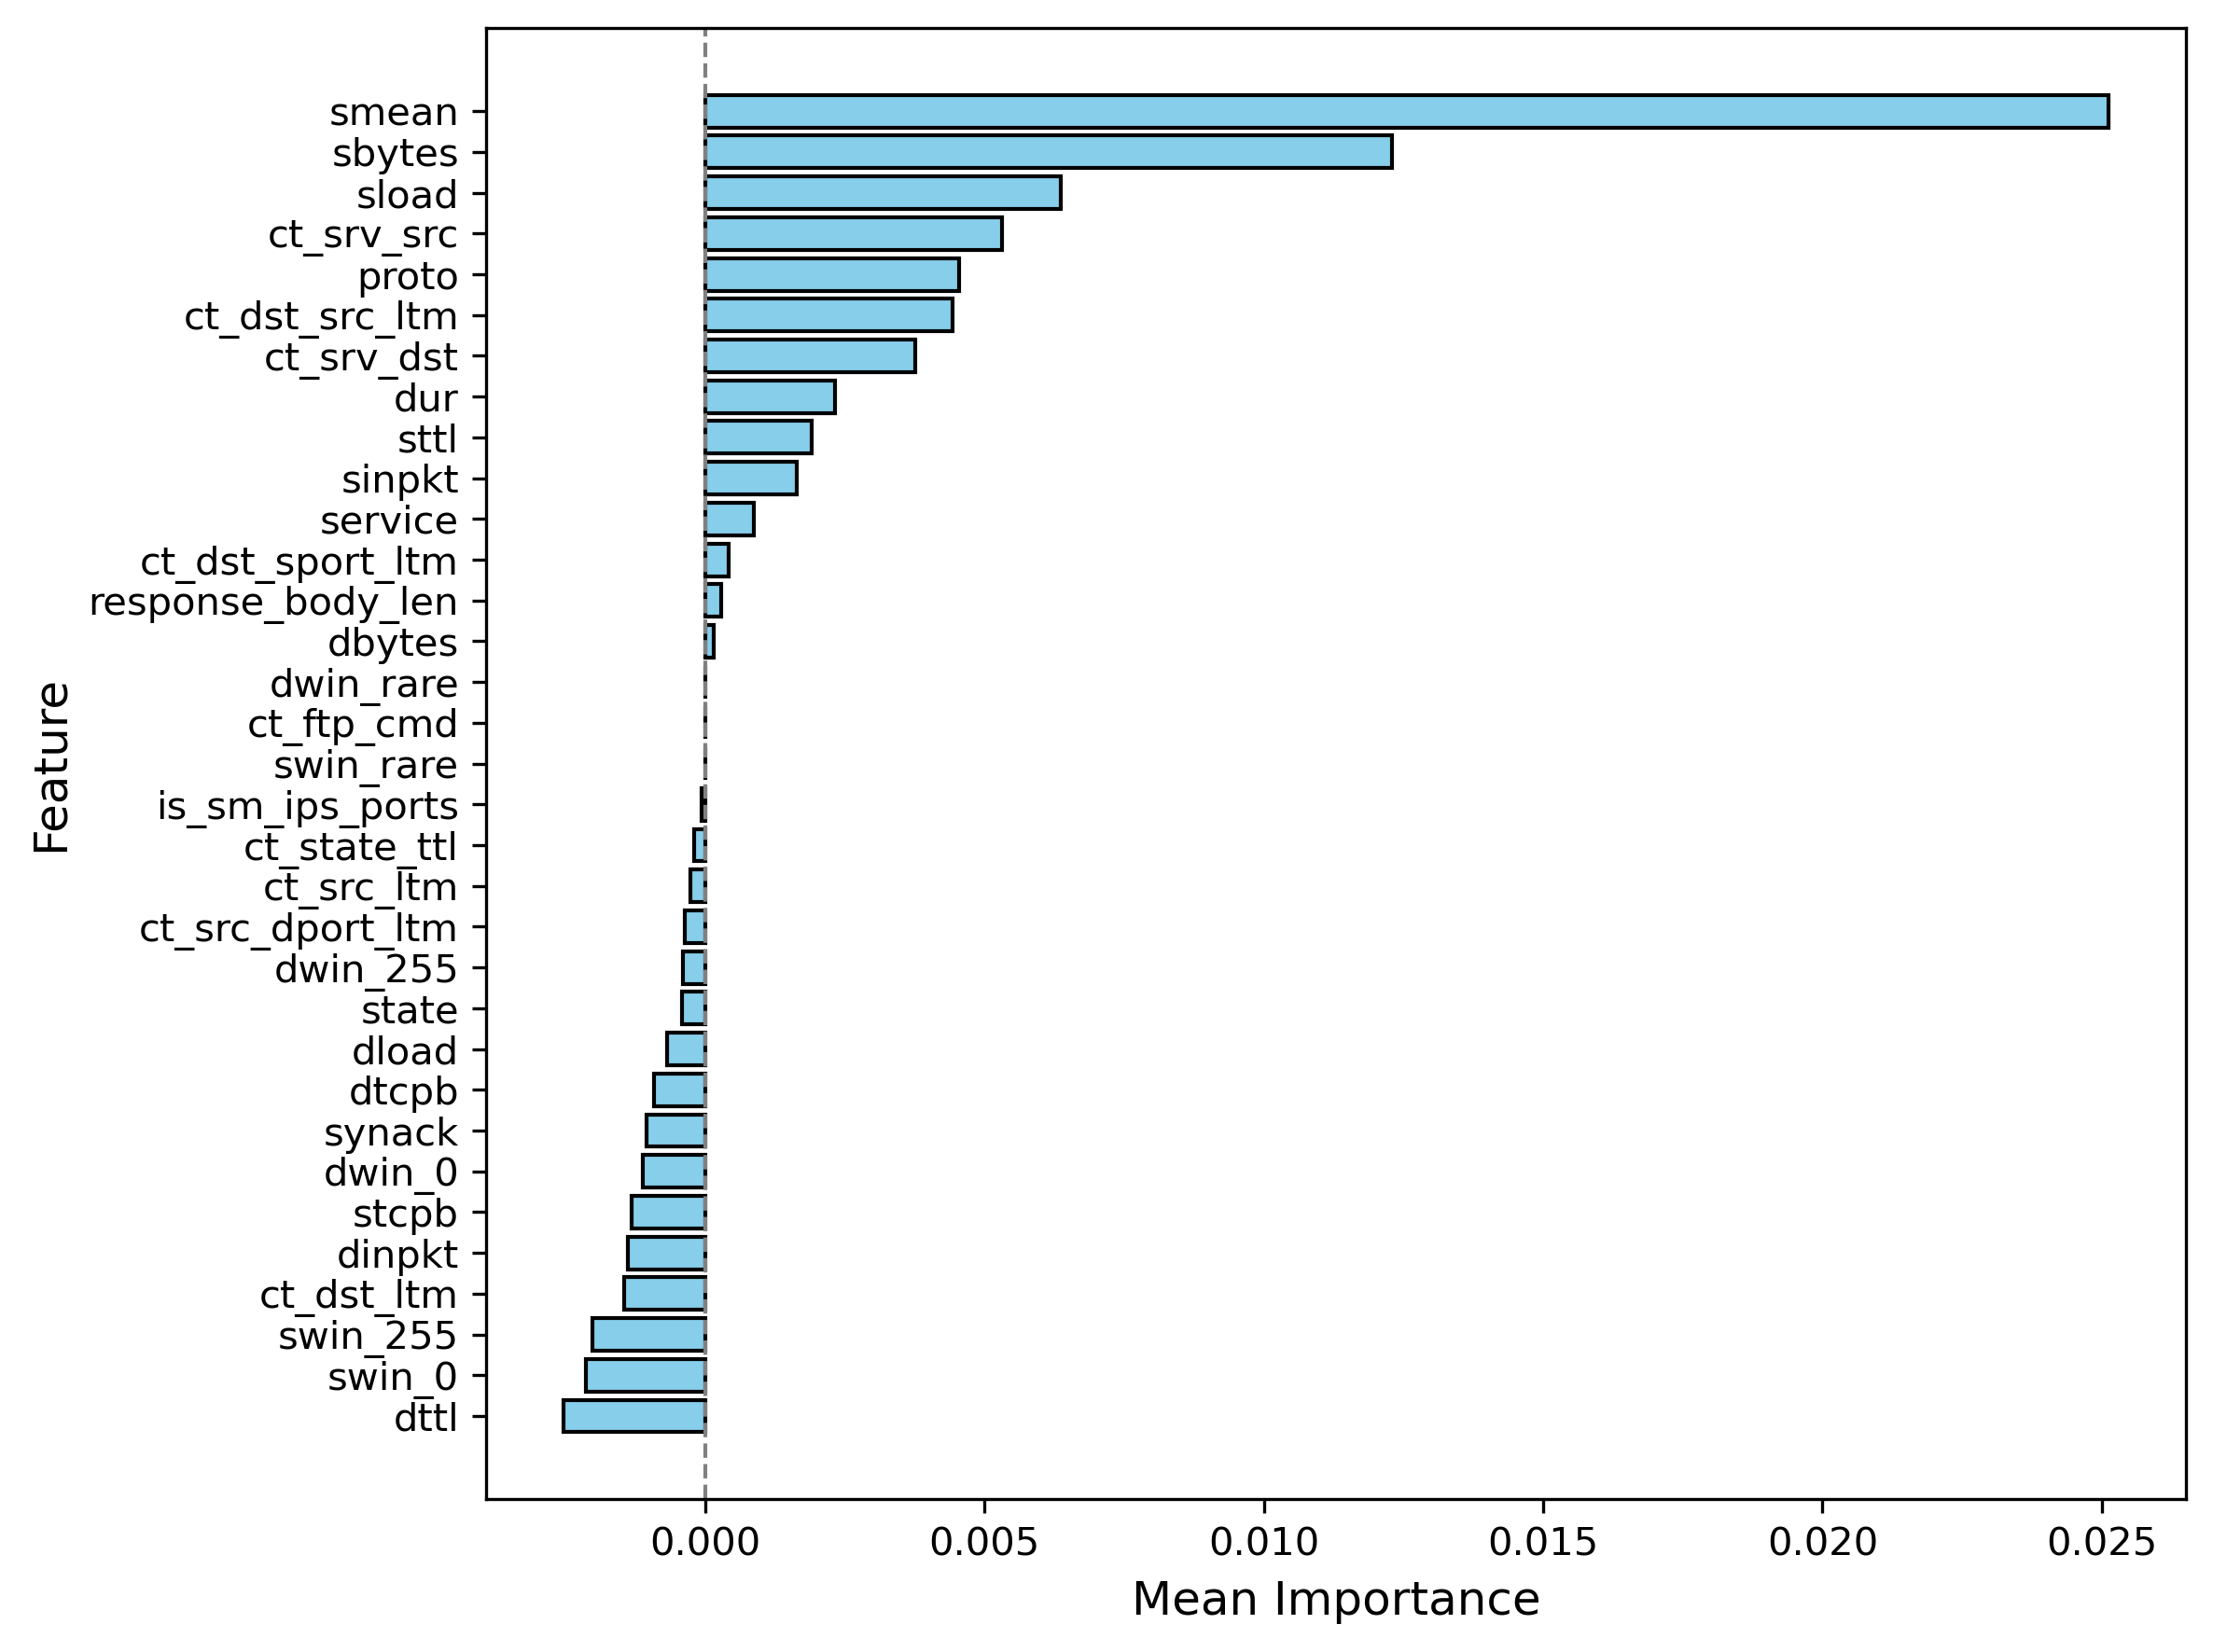
\includegraphics[keepaspectratio]{figures/feature_importance.png}}

}

\caption{\label{fig-importance}Feature importance for the random forest
(RF) classifier.}

\end{figure}%




\end{document}
